\documentclass[a4paper,12pt]{article}
\usepackage{graphicx} 			% Para insertar imagenes
\usepackage{indentfirst} 	% Para sangrar párrafos después de secciones
\setlength{\parindent}{1.5cm} 	% Sangría de 1.5 cm
\usepackage{minted} 	% Para insertar código 
\usepackage{float}
\usepackage[spanish, es-tabla]{babel}
\usepackage{tcolorbox} % Para secciones en destacado
\usepackage{tikz}
\usetikzlibrary{shapes.geometric, arrows.meta, positioning, calc, babel}

\title{Práctica 4: Node.js}
\author{Ángel Rodríguez Faya}
\date{20 de mayo de 2026}

\usepackage{amsmath}
\usepackage{amssymb}

\begin{document}
	
	% --- PÁGINA 1: LA PORTADA ---
	\begin{titlepage}
		\centering
		\vspace*{1cm}
		
		{\huge\bfseries Práctica 4. Node.js \par}
		\vspace{1.5 cm}
		
		{\Large Desarrollo de Sistemas Distribuidos. Grupo DSD-3. \par}
		\vspace{0.25cm}
		{\Large Grado en Ingeniería Informática \par}
		\vspace{0.25cm}
		{\Large Curso 2025-2026.\par}
		\vspace{0.25cm}
		{\Large ETSIIT. Universidad de Granada.\par}
		\vspace{1 cm}
		
		\noindent % Evita la sangría para que aproveche todo el ancho
		\begin{minipage}[c]{0.55\textwidth}
			% La imagen ocupa el 100% del ancho DE ESTA CAJA (no de la hoja)
			
\includegraphics[width=\linewidth]{./imagenes_necesarias/Logotipo_ETSIIT_Horizontal_color.png}
		\end{minipage}% <--- Este % es importante para que no añada espacios extra
		\hfill % Rellena el espacio en medio empujando las cajas a los extremos
		\begin{minipage}[c]{0.40\textwidth}
			\raggedleft % Alinea esta imagen a la derecha dentro de su caja
			
\includegraphics[width=\linewidth]{./imagenes_necesarias/UGR-LOGO-color.png}
		\end{minipage}
		
		\vspace{0.5 cm}
		
		{\large\bfseries Autor: \par}
		{\large Ángel Rodríguez Faya \par}
		\vspace{0.5cm}
		
		{\large\bfseries Profesor: \par}
		{\large José Ángel Segura Muros \par}
		\vspace{1 cm}
		
		{\large\bfseries Fecha de entrega: \par}
		{\large 22 de mayo de 2026\par}
		
	\end{titlepage}
	% El entorno 'titlepage' hace el salto de página automáticamente al cerrar.
	
	% --- PÁGINA 2: EL ÍNDICE ---
	\tableofcontents
	\newpage % <--- Fuerza el salto a la página 3
	
	% --- RESTO DE PÁGINAS:
	
	% ====================================================================
	% 1. INTRODUCCIÓN DE LA MEMORIA
	% ====================================================================
	\section{Introducción.}	
		Este documento constituye la memoria de la Práctica 4 de la asignatura \textit{Desarrollo de Sistemas Distribuidos}. El objetivo central de este proyecto radica en el diseño, implementación y evaluación experimental de un sistema domótico distribuido, cooperativo y en tiempo real, haciendo uso de tres pilares tecnológicos esenciales:
		
		\begin{itemize}
			\item \textbf{Node.js:} Es una plataforma de ejecución de JavaScript del lado del servidor basada en el motor V8 de Google. Destaca por su modelo de operaciones de I/O no bloqueantes y su arquitectura orientada a eventos (\textit{event-driven}), controlada por un único hilo de ejecución centralizado (\textit{Event Loop}). Esto permite mitigar la sobrecarga asociada a la creación de hilos tradicionales por cada conexión entrante.
			
			\item \textbf{Socket.io:} Es una biblioteca especializada en habilitar una capa de comunicación bidireccional, síncrona y de alta velocidad entre clientes y servidores sobre el protocolo WebSocket. Su modelo basado en eventos encaja de forma nativa con el patrón de diseño Publicación/Suscripción, idóneo para la propagación inmediata de estados concurrentes.
			
			\item \textbf{MongoDB:} Es un sistema de base de datos \texttt{NoSQL} orientado a documentos que almacena la información en esquemas flexibles de tipo \texttt{BSON/JSON}. Proporciona un mecanismo de persistencia ideal para el flujo heterogéneo de telemetría y logs de eventos generados de forma asíncrona en entornos distribuidos.
		\end{itemize}
		
		El propósito último de este proyecto/práctica es el despliegue de una infraestructura inteligente donde múltiples procesos independientes — como nodos sensores, nodos actuadores, un agente lógico de control supervisado y paneles web de usuario (o \textit{dashboards})— cooperen de manera asíncrona y transparente para garantizar la habitabilidad y eficiencia del entorno que está siendo monitorizado.
		
		\newpage
		
	% ====================================================================
	% 2. PARTE 1: IMPLEMENTACIÓN DE EJEMPLOS
	% ====================================================================
	\section{Parte 1.- Implementación de ejemplos.}
		Antes de abordar el diseño de la arquitectura completa del sistema domótico, es fundamental que asimilemos los fundamentos de red y los patrones de concurrencia asíncrona que manejan el entorno de Node.js. Por este motivo, la primera fase o parte de la práctica se centra en la implementación, despliegue y análisis de una serie de servicios y ejemplos base propuestos en el guion.
		
		A continuación, vamos a ir viendo cada uno de los ejemplos. Para ello, analizaremos el  código fuente de cada uno de los ejemplos, verificar su correcto funcionamiento mediante capturas de pantalla, y la correspondiente justificación técnica de los fenómenos observados.
		
		\subsection{Ejemplo 1.- Hola Mundo.}
			Para poner en marcha este primer ejemplo, abrimos la terminal en el directorio del archivo (que es \newline \texttt{Parte\_1\_Implementacion\_de\_Ejemplos/Ejemplo\_1\_Hola\_Mundo} ) y ejecutamos el comando:
			\begin{verbatim}
				$ node helloworld.js
			\end{verbatim}
			
			\subsubsection*{Capturas de funcionamiento}
				A continuación se adjuntan las capturas de pantalla que verifican el correcto despliegue del servidor y su respuesta:
				
				\begin{figure}[H]
					\centering
					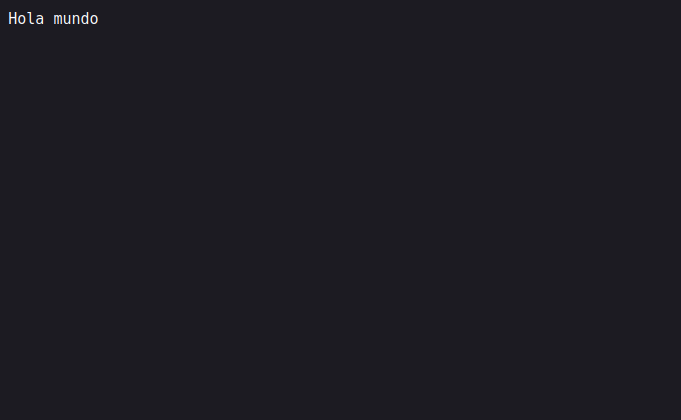
\includegraphics[width=0.8\textwidth]{./imagenes_necesarias/ejemplos_ejecucion/parte_1/ejemplo1_1.png}
					\caption{Visualización en el navegador de la respuesta enviada por el servidor.}
					\label{fig:ejemplo1_navegador}
				\end{figure}
				
				\begin{figure}[H]
					\centering
					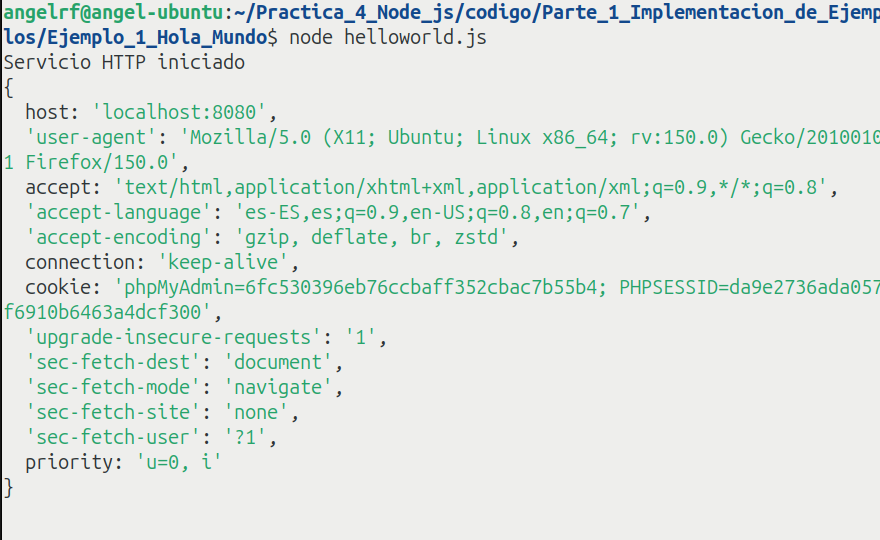
\includegraphics[width=0.8\textwidth]{./imagenes_necesarias/ejemplos_ejecucion/parte_1/ejemplo1_2.png}
					\caption{Salida por terminal del servidor mostrando el inicio y las cabeceras recibidas.}
					\label{fig:ejemplo1_terminal}
				\end{figure}
				
				Vemos que el script utiliza el módulo nativo \texttt{http} de Node.js para levantar un servidor web básico que se queda escuchando peticiones en el puerto \texttt{8080}. Cada vez que un cliente (como el navegador) accede, el servidor imprime en la consola las cabeceras de la petición y devuelve un mensaje de texto plano con el contenido ``Hola mundo''.
				
				Lo más relevante a destacar de este ejemplo es:
				\begin{itemize}
					\item \textbf{La petición no bloqueante (Asíncrona):} El mensaje \texttt{'Servicio HTTP iniciado'} se muestra en la terminal de forma inmediata al lanzar el script. Esto demuestra que el método \texttt{.listen(8080)} es asíncrono y no detiene la ejecución del programa a esperar conexiones.
					\item \textbf{Uso de Callbacks:} La función interna de \texttt{createServer} actúa como un \textit{callback}. No se ejecuta al arrancar el programa, sino que el \textit{Event Loop} (bucle de eventos) la invoca únicamente cuando entra una petición HTTP, gestionando así la concurrencia de forma eficiente en un solo hilo o hebar.
				\end{itemize}

		\subsection{Ejemplo 2.- Calculadora REST.}
			Para este segundo ejemplo, lo podemos poner en marcha abriendo en la terminal el directorio del archivo (que es \newline \texttt{Parte\_1\_Implementacion\_de\_Ejemplos/Ejemplo\_2\_Calculadora\_REST} ) y ejecutamos el comando:
			
			\begin{verbatim}
				$ node calculadora.js
			\end{verbatim}
			
			\subsubsection*{Capturas de funcionamiento}
				A continuación se adjuntan las capturas de pantalla:
				
				\begin{figure}[H]
					\centering
					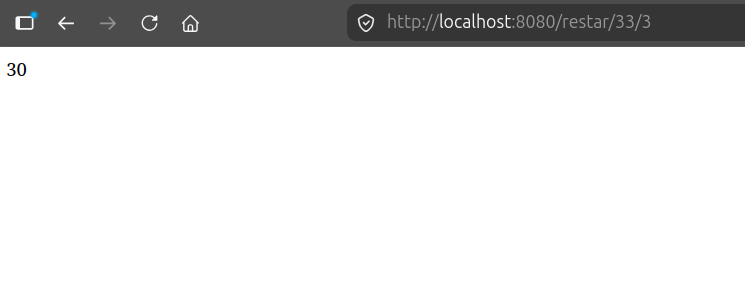
\includegraphics[width=0.8\textwidth]{./imagenes_necesarias/ejemplos_ejecucion/parte_1/ejemplo2_1.png}
					\caption{Visualización en el navegador del resultado de restar 33-3}
					\label{fig:ejemplo2_navegador}
				\end{figure}
				
				\begin{figure}[H]
					\centering
					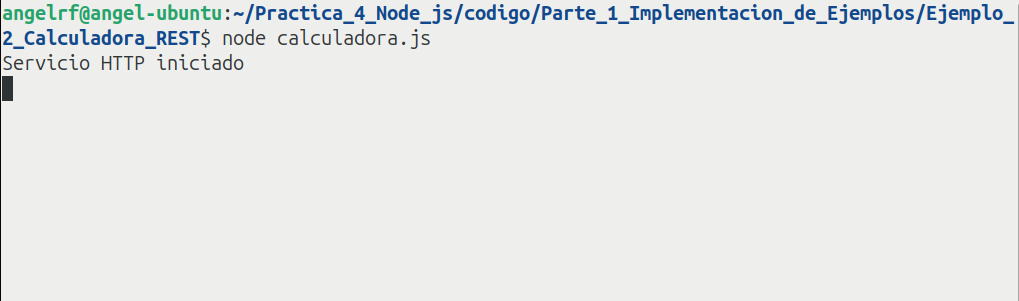
\includegraphics[width=0.8\textwidth]{./imagenes_necesarias/ejemplos_ejecucion/parte_1/ejemplo2_2.png}
					\caption{Salida por terminal del servidor mostrando el inicio.}
					\label{fig:ejemplo2_terminal}
				\end{figure}
				
				Viendo el código fuente y la figura~\ref{fig:ejemplo2_navegador} podemos sacar varias conclusiones/apuntes sobre Node.js:
				\begin{itemize}
					\item El servidor tiene que \textbf{procesar la URL} como una cadena de texto, para descomponer la ruta de la petición en un array de parámetros. 
					
					\item Como todo lo que viaja por HTTP es texto, necesitamos \textbf{deserializar los datos }mediante \texttt{parseFloat()} para operar con ellos numéricamente y, posteriormente, convertirlos de nuevo a texto (\texttt{result.toString()}) para poder transmitirlos en la respuesta HTTP.
					
					\item Se realiza un \textbf{control de errores}. Se comprueba que el array de parámetros extraído de la URL tenga $>= 3$ parámetros para poder realizar la operación. En caso de que tenga menos, el sistema no se cae (no hace \textit{crash}), si no que responde con un mensaje de error controlado manteniendo así la \textbf{disponibilidad del servicio}
				\end{itemize}
				
				Este ejemplo es una calculadora \textbf{REST}. Esto quiere decir que el servidor actúa como una \textbf{API}. Solo espera recibir comandos en la URL (ej. /sumar/5/3) y devuelve datos puros (el resultado en texto plano). No tiene diseño, ni botones, ni colores. Está pensado para comunicación máquina a máquina (por ejemplo, para que otro programa o un comando de terminal interactúe con él), tal y cómo hemos visto en las capturas de pantalla.

		\subsection{Ejemplo 3.- Calculadora WEB.}
			En este ejemplo, vemos otra calculadora pero a diferencia de la anterior, esta es una calculadora WEB. Es decir, el servidor actúa como un \textbf{Servidor Web tradicional y además como API}. Está orientado a humanos y no a máquinas como el ejemplo anterior. Cuando entras a la ruta base (/), el servidor lee del disco duro y nos devuelve una página web completa (\texttt{calc.html}). Esa página web tiene una interfaz visual (un formulario, un desplegable) y contiene código JavaScript que, de forma invisible (usando peticiones \texttt{fetch}), hace las llamadas REST al servidor para obtener el resultado sin tener que recargar la página.
			
			Para poder ejecutar este ejemplo, abrimos la terminal y nos situamos en el directorio del archivo (que es \newline \texttt{Parte\_1\_Implementacion\_de\_Ejemplos/Ejemplo\_3\_Calculadora\_WEB} ) y ejecutamos el comando:
			
			\begin{verbatim}
				$ node calculadora-web.js
			\end{verbatim}
			
			\subsubsection*{Capturas de funcionamiento}
				A continuación se adjuntan las capturas de pantalla:
				
				\begin{figure}[H]
					\centering
					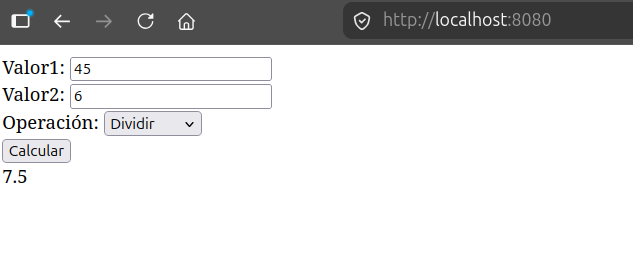
\includegraphics[width=0.8\textwidth]{./imagenes_necesarias/ejemplos_ejecucion/parte_1/ejemplo3_1.png}
					\caption{Visualización en el navegador de la calculadora comportándose como una página web normal. Divide $45/6$.}
					\label{fig:ejemplo3-1_navegador}
				\end{figure}
				
				\begin{figure}[H]
					\centering
					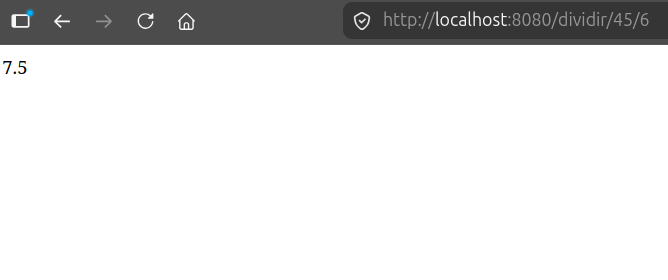
\includegraphics[width=0.8\textwidth]{./imagenes_necesarias/ejemplos_ejecucion/parte_1/ejemplo3_2.png}
					\caption{Visualización en el navegador de la calculadora comportándose como una API. Divide $45/6$.}
					\label{fig:ejemplo3-2_navegador}
				\end{figure}
				
				\begin{figure}[H]
					\centering
					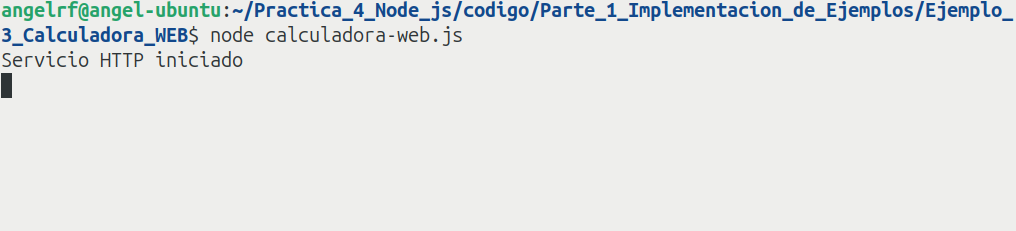
\includegraphics[width=0.8\textwidth]{./imagenes_necesarias/ejemplos_ejecucion/parte_1/ejemplo3_3.png}
					\caption{Salida por terminal del servidor mostrando el inicio.}
					\label{fig:ejemplo3_terminal}
				\end{figure}
				
				Este ejemplo da un paso más hacia una arquitectura web real al separar el \textit{Frontend} (interfaz) del \textit{Backend} (lógica). El servidor ahora realiza dos funciones distintas dependiendo de la ruta (\textit{routing}) solicitada:
				
				\begin{itemize}
					\item  En la figura ~\ref{fig:ejemplo3-1_navegador} podemos ver el \textbf{servicio de archivos estáticos (I/O Asíncrono)}. Si el cliente accede a la raíz (\texttt{/}), el servidor utiliza los módulos nativos \texttt{path} y \texttt{fs} (File System) para buscar el archivo \texttt{calc.html} en el disco duro. Emplea la función asíncrona \texttt{readFile} junto con un \textit{callback} \texttt{(err, data)} para leer el archivo sin bloquear el hilo principal, y lo devuelve al cliente con la cabecera \texttt{text/html}. Comportándose como una página web real.
					
					\item En cambio, en la figura ~\ref{fig:ejemplo3-2_navegador}, vemos en acción el \textbf{consumo de API mediante AJAX (\texttt{fetch}).} En el lado del cliente (el navegador), el archivo HTML contiene un script que intercepta el envío del formulario (\texttt{submit}). En lugar de recargar la página, utiliza la API \texttt{fetch} de JavaScript (basada en Promesas con \texttt{.then()}) para construir la URL dinámica (ej. \texttt{/sumar/5/3}), solicitar el resultado al servidor en segundo plano y actualizar únicamente la etiqueta \texttt{<span>} del resultado en el DOM. Este comportamiento es parecido al de la calculadora del ejemplo anterior.
				\end{itemize}

		\subsection{Ejemplo 4.- Socket.io.}
			Ahora ya estamos ante una página web \textbf{en tiempo real y bidireccional}. En este ejemplo voy a comentar primero las anotaciones o cueriosidades y luego vemos los ejemplos.
			
			\begin{itemize}
				 
			\item  Ya nos olvidamos de las peticiones, pues ahora trabajaremos con \textbf{eventos}. Esto ocurre porque, a diferencia de  HTTP que obliga a que el navegador siempre pregunte primero para que el servidor responda, Socket.io (basado en WebSockets) mantiene un "tubo" de comunicación siempre abierto. Ahora, el servidor puede enviar datos al navegador por iniciativa propia sin que nadie se lo pida.
			
			\item Estamos ante el \textbf{Patrón de Suscripción/Emisión} (\texttt{emit} y \texttt{on}), que se diferencia con el \textbf{Patrón \textit{Observer}} en que los publicadores (emisores) y los suscriptores (receptores) no se comunican directamente entre sí. Utilizan un intermediario (\textit{Message Broker} o Bus de Eventos). Los publicadores envían mensajes a un "canal" o "tema" y los suscriptores escuchan ese canal.
			Es por eso que la comunicación ya no se basa en URLs (rutas), sino en "eventos" con nombres inventados por el programador.
			\begin{itemize}
				\item  Usamos \texttt{.emit('nombre-evento', datos)} para disparar un mensaje por el "tubo".
				
				\item Usamos \texttt{.on('nombre-evento', callback)} para quedarnos escuchando.
				
				\item Por ejemplo, el navegador emite \texttt{output-evt} con el texto "¡Hola Servicio!", y el servidor lo escucha para contestar.
			\end{itemize}
			
			\item Se realiza una\textbf{ Difusión o \textit{Broadcast}} (\texttt{io.sockets.emit}): El servidor de Node.js guarda un array llamado \texttt{allClients} con las direcciones IP y puertos de todos los conectados. Cuando alguien nuevo entra (o cuando alguien cierra la pestaña y se dispara el evento \texttt{disconnect}), el servidor usa \texttt{io.sockets.emit('all-connections', allClients}), para mantenerla lista actualizada a todos los clientes que están conectados a la vez.
			
			\item El \textbf{DOM es Dinámico} (Frontend): En el archivo HTML, encontramos código JavaScript que está "suscrito" al evento \texttt{all-connections}. Cada vez que el servidor lanza esa nueva lista, el cliente borra la lista antigua de la pantalla y dibuja la nueva al instante, sin tener que darle al botón de actualizar del navegador.
			
		\end{itemize}
		
		Para poder ejecutar este ejemplo, abrimos la terminal y nos situamos en el directorio del archivo (que es \newline \texttt{Parte\_1\_Implementacion\_de\_Ejemplos/Ejemplo\_4\_Socketio} ) y ejecutamos el comando:
			
		\begin{verbatim}
			$ node connections.js 
		\end{verbatim}
		
		\subsubsection*{Capturas de funcionamiento}
			A continuación se adjuntan las capturas de pantalla:
			
			\begin{figure}[H]
				\centering
				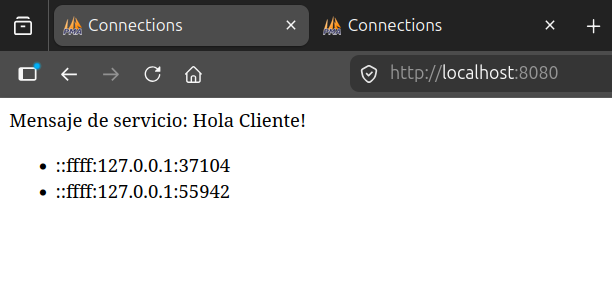
\includegraphics[width=0.8\textwidth]{./imagenes_necesarias/ejemplos_ejecucion/parte_1/ejemplo4_1.png}
				\caption{Visualización en el navegador de la dirección Ip y el puerto de los dos clientes conectados a nuestro servidor.}
				\label{fig:ejemplo4_navegador}
			\end{figure}
			
			\begin{figure}[H]
				\centering
				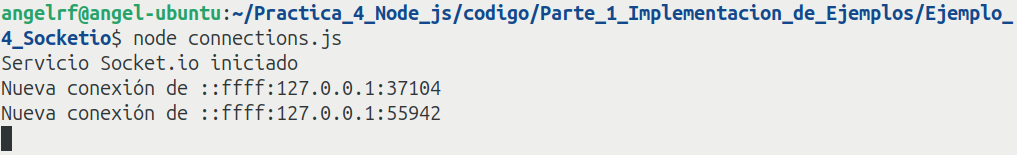
\includegraphics[width=0.8\textwidth]{./imagenes_necesarias/ejemplos_ejecucion/parte_1/ejemplo4_2.png}
				\caption{Salida por terminal del servidor mostrando el inicio.}
				\label{fig:ejemplo4_terminal}
			\end{figure}
			
			Como podemos observar en las figuras, el cliente web muestra los clientes conectados. La dirección IP es la misma puesto que he abierto dos pestañas en mi misma máquina, eso sí, el puerto obviamente si que cambia
				
		\subsection{Ejemplo 5.- MongoDB.}
			En este ejemplo vamos un paso más allá: incorporar una base de datos real. Utilizaremos \texttt{MongoDB}, que es un sistema de gestión de bases de datos de tipo NoSQL . Este SGBD utiliza colecciones de entradas en formato JSON, en lugar de tablas que encontramos en SQL. Cada entrada puede tener un conjunto de claves y valores arbitrarios. Para obtener información, realizamos consultas similares a las utilizadas en SQL.
			
			En este caso se utiliza para almacenar los clientes que se han conectado en nuestro servidor. En el ejemplo 4, los clientes conectados se almacenaban en un array de JS. Tenía como inconveniente que los datos eran volátiles, pues cuando apagamos el servidor, el array obviamente se borraba. En este ejemplo, podemos ver en las capturas de pantalla que las direcciones de los clientes se almacenan en la BD, porque se almacenan junto a la fecha y hora en la que se conectaron, y vemos que hay dos fechas distintas: 24 de abril y 21 de mayo.
			
			Para poder ejecutar este ejemplo, abrimos la terminal y nos situamos en el directorio del archivo (que es \newline \texttt{Parte\_1\_Implementacion\_de\_Ejemplos/Ejemplo\_5\_MongoDB} ) y ejecutamos los comandos:
			
			\begin{itemize}
				\item Para arrancar el servicio de MongoDB (previamente debe estar instalado en nuestro PC)
					\begin{verbatim}
						$ sudo systemctl start mongod
					\end{verbatim}
					
				\item Para lanzar el servidor:
					\begin{verbatim}
						$ node mongo-test.js
					\end{verbatim}
				
			\end{itemize}

			\begin{figure}[H]
				\centering
				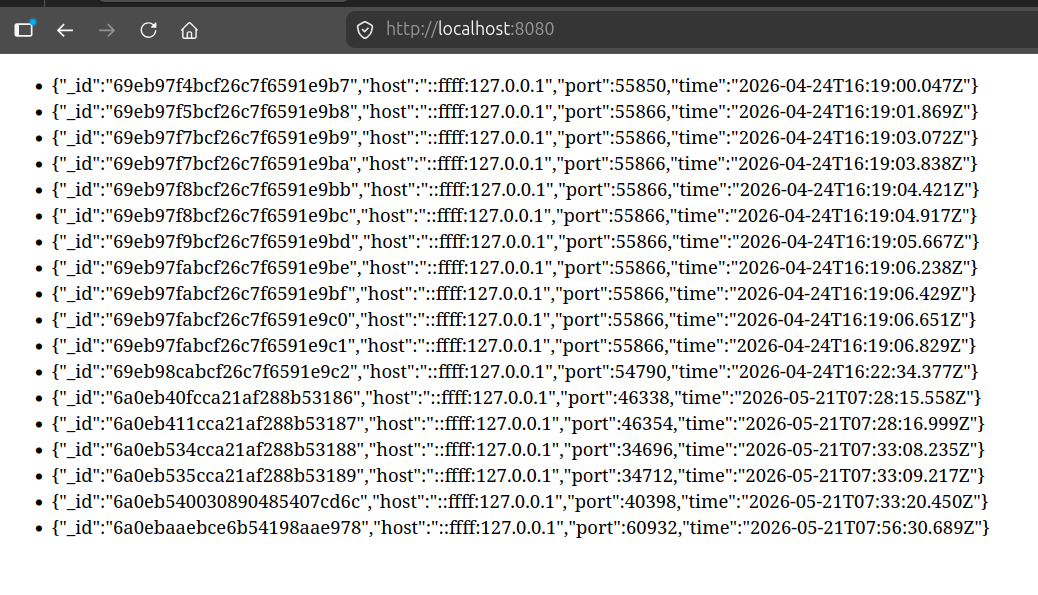
\includegraphics[width=0.8\textwidth]{./imagenes_necesarias/ejemplos_ejecucion/parte_1/ejemplo5_1.png}
				\caption{Visualización en el navegador de os clientes que se han conectado alguna vez al servidor.}
				\label{fig:ejemplo5_navegador}
			\end{figure}
			
			\begin{figure}[H]
				\centering
				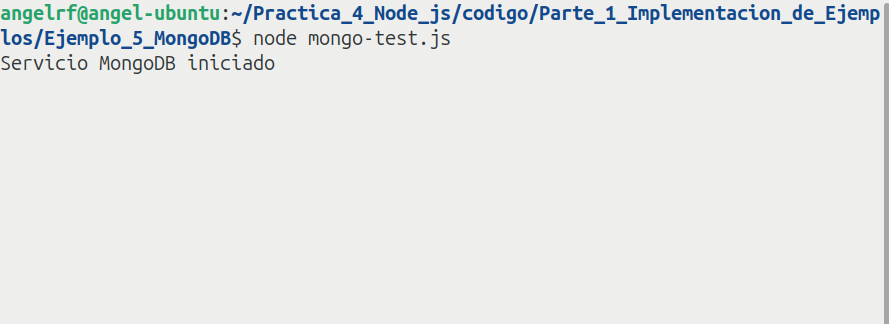
\includegraphics[width=0.8\textwidth]{./imagenes_necesarias/ejemplos_ejecucion/parte_1/ejemplo5_2.png}
				\caption{Salida por terminal del servidor mostrando el inicio.}
				\label{fig:ejemplo5_terminal}
			\end{figure}
			
			Observando las figuras ~\ref{fig:ejemplo5_navegador} y ~\ref{fig:ejemplo5_terminal}, vemos que, a diferencia del Ejemplo 4 (donde solo imprimíamos texto plano formateado con la IP y el puerto), aquí vemos que los datos aparecen en pantalla como objetos JSON puros encadenados. El campo llamado \texttt{\_id} con un código alfanumérico largo (\texttt{ObjectId}). Este elemento no lo ha programado el cliente; lo genera e inyecta MongoDB automáticamente para que actúe como clave primaria única del documento dentro de la colección.
			
			Además, se utilizan Promesas o \textit{Promises} para un \textit{Flujo Asíncrono} , evitando bloquear el único hilo de ejecución de Node.js durante las operaciones de Entrada/Salida (I/O) con el disco. El driver de MongoDB utiliza las \textit{Promises}. Toda la lógica de red se anida secuencialmente dentro de métodos \texttt{.then()}, asegurando que el servidor pueda seguir escuchando nuevos sockets mientras procesa consultas concurrentes.
			
			En el Ejemplo 4, el servidor tomaba un rol activo enviando la lista de conexiones por iniciativa propia nada más establecerse el enlace. En el Ejemplo 5, el flujo lo conduce el cliente web de forma reactiva: 
			\begin{enumerate}
				\item El servidor le dice al cliente cuál es su dirección (\texttt{my-address}).
				\item El cliente añade la fecha actual y ordena activamente guardarla (\texttt{poner}).
				\item Finalmente, el cliente solicita expresamente recuperar el histórico (\texttt{obtener}).
			\end{enumerate}
			
			Por último, destacar que el Servidor no tiene estado (\textit{Stateless}). Es lo que habíamos comentado al principio del ejemplo, dado que el servidor de Node.js ya no mantiene ninguna lista viva de sockets en su memoria volátil, se elimina por completo la necesidad de escuchar el evento \texttt{disconnect} en \texttt{mongo-test.js}. Al servidor le resulta indiferente si el usuario cierra el navegador, ya que el registro queda guardado de manera permanente e inmutable en MongoDB.
	
	\newpage
	% ====================================================================
	% 3. PARTE 2: S	istema domótico
	% ====================================================================
	\section{Parte 2.- Sistema Domótico.}
		
		\subsection{Introducción}
		
			El objetivo de esta segunda parte de la práctica radica en el diseño, implementación y evaluación experimental de un sistema domótico distribuido, cooperativo y en tiempo real, haciendo uso de los pilares tecnológicos que ya comentamos en la sección anterior:  \textbf{Node.js}, \textbf{Socket.io} y \textbf{MongoDB}. 
			
			El motivo de realizar esta parte sobre un sistema domótico es la de simular el despliegue de una infraestructura inteligente donde múltiples procesos independientes cooperen de manera asíncrona y transparente. Para ello, el sistema se ha diseñado cumpliendo los siguientes requisitos y características arquitectónicas:
		
			\begin{enumerate}
				\item \textbf{Emulación de Nodos Sensores y Actuadores:} Creación de clientes web independientes que actúan como sensores físicos (Temperatura, Luminosidad, Gas, Movimiento y Videovigilancia), publicando telemetría tanto de forma periódica (5 segundos), como de forma manual; hacia el servidor central.
				
				\item \textbf{Agente Lógico Centralizado:} Implementación de un motor de reglas en el servidor que evalúa la telemetría entrante en tiempo real para tomar decisiones sobre los actuadores (ej. encender el aire acondicionado, bajar persianas o activar alarmas de gas). Se incluyen tanto reglas simples puramente reactivas, como \textbf{reglas complejas con memoria} (ej. mantener las luces encendidas un tiempo determinado tras dejar de detectar movimiento).
				
				\item \textbf{Patrón de ``Gemelo Digital'':} El servidor mantiene una representación en memoria (\textit{Digital Twin}) del estado físico real de los actuadores por zonas de la casa, asegurando la consistencia de los datos y evitando ''fantasmas'' en la interfaz web`. Un \textbf{Gemelo Digital} (\textit{Digital Twin}) es una réplica virtual de un objeto, sistema o proceso físico del mundo real. No es solo un dibujo o un modelo estático en 3D; \textbf{es una representación informática dinámica que se actualiza en tiempo real utilizando los datos que envían los sensores del mundo físico.}
				
				\item \textbf{Panel de Control (Dashboard):} Una interfaz web central, separada de la lógica de negocio y diseñada para el \textbf{usuario} , que se actualiza reactivamente mediante \textit{broadcast} mostrando la lectura de los sensores, el estado de los actuadores y un registro de alertas críticas, así como un panel que muestra en tiempo real el \textbf{Circuito Cerrado de Videovigilancia}.
				
				\item \textbf{Telegram Bot API.} Se ha desarrollado una Plataforma de integración a través de peticiones HTTP REST que permite expandir los límites físicos del sistema domótico, enviando alertas críticas (al igual que en el \textit{Dashboard}) y contenido multimedia del Circuito de Videovigilancia directamente al dispositivo del usuario de forma instantánea.
			\end{enumerate}
			
			Con estas implementaciones añadidas (además de la implementación básica), se cubren todos los requisitos que se piden en el guion de prácticas. A continuación, se detalla la arquitectura del sistema y su modelo de funcionamiento.
			
		\subsection{Arquitectura del Sistema}
		
			El sistema domótico se ha diseñado siguiendo un patrón de arquitectura \textit{Cliente-Servidor Distribuido} y \textit{Orientado a Eventos}. La comunicación principal se basa sobre conexiones persistentes de baja latencia mediante el protocolo WebSocket (gestionado a través de \textit{Socket.io}), rompiendo con el esquema tradicional de petición/respuesta síncrona de HTTP. 
			
			A continuación, se desglosan los componentes del sistema divididos de forma lógica entre el núcleo central (Servidor) y los procesos periféricos (Clientes).
			
			\subsubsection{El Servidor Central (\texttt{registro\_sensores.js})}
				El servidor central  actúa como el cerebro de toda la casa inteligente (es el \textbf{Bus de Evnetos} y el \textbf{Agente Lógico} que toma las decisiones). Sus tareas principales dentro de nuestro sistema son las siguientes:
				
				\begin{itemize}
					\item \textbf{Atender a los clientes:} Escucha en el puerto \texttt{8080} y mantiene abiertas las conexiones en tiempo real (mediante WebSockets) con todos los dispositivos. Además, es capaz de identificar si el que se ha conectado es un sensor enviando datos o es el panel de control del usuario.
					
					\item \textbf{Mantener el ``Gemelo Digital'':} Para evitar fallos o desincronizaciones, el servidor guarda en su propia memoria una copia exacta (un reflejo) del estado actual de todos los actuadores de la casa (luces, persianas, etc.). Cualquier cambio pasa primero por aquí.
					
					\item \textbf{Tomar decisiones (Agente Lógico):} Analiza al vuelo cada dato que le llega de los sensores. Si detecta algo fuera de lo normal (por ejemplo, que el nivel de gas supera los 300 o que hay movimiento en el portal), ejecuta automáticamente las reglas que hemos programado para lanzar alertas o cambiar el estado de los actuadores.
					
					\item \textbf{Guardar el historial:} Utiliza la base de datos de \texttt{MongoDB} para ir anotando todo lo que ocurre. Lo hace de forma asíncrona (usando Promesas), lo que significa que el servidor puede seguir guardando registros sin quedarse "congelado" ni desatender al resto de la casa.
				\end{itemize}
				
				Su código es el siguiente:
				
				%\inputminted[linenos, frame=lines, fontsize=\scriptsize]{JavaScript}{../codigo/Parte_2_Sensores_Domoticos/registro_sensores.js}
				
				Para entender cómo funciona este servidor más allá de los comentarios de su código, podemos destacar cinco bloques de implementación clave que estructuran su lógica:
				
				\begin{itemize}
					\item \textbf{Definición Estricta de Estados y Gemelo Digital:} Se hace uso de \texttt{Object.freeze} para definir los estados de los actuadores (como \texttt{ENCENDIDO}, \texttt{APAGADO}, \texttt{ABIERTA} o \texttt{CERRADA}) de forma inmutable. Esto evita errores de escritura en el código. Estos estados se agrupan en el objeto global \texttt{estadoActuadores}, que actúa como el \textit{Digital Twin} en memoria. Cada vez que una interfaz se conecta, lo primero que hace el servidor es enviarle este objeto para asegurar que el usuario vea exactamente lo que está pasando en la casa.
					
					\item \textbf{Servidor HTTP Nativo :} El servidor lee los archivos HTML directamente desde el disco (\textit{sensor.html} y \textit{dashboard.html}) y los sirve según la ruta que pida el navegador, manejando los errores de carga manualmente.
					
					\item \textbf{Gestión de Eventos Bidireccionales (Socket.IO):} El corazón de la comunicación en tiempo real se divide en dos tipos de eventos bien diferenciados:
					\begin{itemize}
						\item \textit{Eventos de entrada (\texttt{sensor:data}):} Reciben las lecturas, las guardan en la colección \texttt{historial} de MongoDB y las reenvían al instante a los paneles de control mediante un \texttt{broadcast} global (\texttt{io.sockets.emit}).
						
						\item \textit{Eventos de control manual (\texttt{ui:toggle-*}):} Escuchan las órdenes directas que el usuario pulsa en el Dashboard (como encender el aire o bajar una persiana), modifican el Gemelo Digital en el servidor y vuelven a avisar a todas las pantallas abiertas para que se actualicen a la vez.
					\end{itemize}
					
					\item \textbf{El Agente Lógico:} La función \texttt{ejecutarAgente} centraliza la inteligencia del sistema evaluando los umbrales críticos. Encontramos tanto reglas puramente reactivas (apagar el aire si la temperatura baja de 17°C) como \textbf{reglas complejas con memoria}. Un ejemplo claro es la regla de movimiento, que consulta primero el objeto \texttt{memoriaLuminosidad} para comprobar si la última lectura de luz era baja (< 200 lux), evitando así encender bombillas de forma innecesaria durante el día. Otra curiosidad de este agente es que, dependiendo de si la ubicacion de la medida que se pasa como parámetro tiene un actuador para ese sensor o no, se gestiona de una forma u otra. Esto hace que, si nosotros queremos registrar un nuevo sensor(por ej: un sensor de gas en el baño), no nos ponga ningún inconveniente y por tanto, cada vez que se detecte una anomalía se nos notificará en forma de aviso mediante el \textit{Dashboard} y por el bot de Telegram (\textbf{DomoBot Angel}). Ahora bien, como en el Gemelo Digital (\texttt{estadoActuadores}) no hay definido un actuador para el gas en la ubicación de Baño, no se activará la correspondiente alarma y sólo nos llegará el aviso. \textbf{Con esto, se pretende hacer ver que, podemos añadir tantos sensores como queramos y de varios tipos, pero dependiendo de si tienen actuadores o no, se adaptarán las salidas}.
						
						\item \textbf{DomoBot Angel} (El bot de Telegram): Como ya hemos comentado, DomoBot Angel~\ref{fig:DomoBot Angel} es el bot que nos avisa sobre lo que está sucediendo en nuestro hogar, por si no podemos acceder en ese momento al \textit{Dashboard}. Es importante saber que \textbf{sólo sirve para notificar, NO para actuar}, es decir, el bot nos muestra avisos sobre anomalías detectadas por nuestros sensores, pero no es posible acceder a los actuadores, para eso hay que acceder al Dashboard. A pesar de esto, no deja de ser un añadido atractivo e importante en el proyecto.
						
						\begin{figure}[H]
							\centering
							
\includegraphics[width=0.8\textwidth]{./imagenes_necesarias/ejemplos_ejecucion/parte_2/DomoBot_Angel_1.png}
							\caption{Imagen sobre DomoBot Angel.}
							\label{fig:DomoBot Angel}
						\end{figure}
					\end{itemize}

			\subsubsection{Nodos Sensores y Emulación (\texttt{sensor.html})}
				Los sensores son los "ojos" y "oídos" de la casa domotizada. Este cliente web está diseñado para emular el comportamiento de un hardware IoT real, y sus tareas principales son:
				
				\begin{itemize}
					\item \textbf{Dar de alta el dispositivo:} Permite al usuario registrar un nuevo sensor indicando su nombre, en qué ubicación de la casa está y de qué tipo es (Luminosidad, Gas, Videovigilancia, etc.).
					\item \textbf{Escoger un dispositivo existente:} Además de poder añadir sensores nuevos, también se puede acceder a los que ya están creados (y almacenados en la colección \texttt{sensores} de nuestra base de datos en MongoDB).
					\item \textbf{Envío manual de datos:} Tiene un formulario para poder inyectar valores concretos al servidor y comprobar cómo reacciona el sistema (ideal para hacer pruebas de umbrales críticos).
					\item \textbf{Simulación automática (Modo Piloto Automático):} Es capaz de generar ráfagas continuas de datos aleatorios realistas y enviarlos al servidor de forma constante sin intervención humana. En el código, está fijado a 5000 milisegundos (5 segundos)
				\end{itemize}
				
				Su código es el siguiente:
				
			%	\inputminted[linenos, frame=lines, fontsize=\scriptsize]{HTML}{../codigo/Parte_2_Sensores_Domoticos/sensor.html}
				
				Más allá de la estructura visual en HTML y CSS, la verdadera lógica de este cliente reside en su script de JavaScript. Podemos destacar los siguientes bloques clave en su implementación:
				
				\begin{itemize}
					\item \textbf{Validación y Registro Dinámico:} Antes de enviar nada, el cliente comprueba que los campos obligatorios del formulario estén completos. Si todo es correcto, emite el evento \texttt{sensor:register} y el servidor se encarga de guardarlo en MongoDB. Además, al cargar la página, el cliente pide al servidor la lista de sensores que ya existen en la base de datos para mostrarlos en un desplegable, evitando duplicados.
					
					\item \textbf{Motor de Simulación Automática:} Mediante la función \texttt{setInterval}, hemos creado un bucle que se repite cada 5 segundos, como ya hemos comentado. Dentro de este bucle, un bloque \texttt{switch} analiza de qué tipo es el sensor seleccionado y genera datos matemáticamente creíbles (por ejemplo, temperaturas con decimales entre 7ºC y 35ºC, o valores binarios 0/1 para el movimiento o la cámara). Esto satura de eventos al servidor para probar su rendimiento real.
					
					\item \textbf{Desacoplamiento Visual/Lógico:} El envío de datos (\texttt{enviarMedidaAlServidor}) está programado en una función independiente. Esto permite que tanto el botón manual como el bucle automático reciclen el mismo código para comunicarse con el servidor, manteniendo el script limpio.
				\end{itemize}

			\subsubsection{Panel de Control de Usuario (\texttt{dashboard.html})}
				Es la interfaz visual diseñada para los habitantes de la casa. A diferencia de una página web tradicional que requiere recargarla para ver los cambios, este panel es una aplicación \textbf{100\% reactiva y asíncrona}. Sus tareas principales son:
				
				\begin{itemize}
					\item \textbf{Monitorización en tiempo real:} Muestra las últimas lecturas de todos los sensores activos de la casa y el registro de alertas críticas.
					\item \textbf{Control interactivo:} Ofrece botones para que el usuario pueda manejar los actuadores (encender o apagar luces, aires acondicionados y alarmas) manualmente
					\item \textbf{CCTV Multimedia:} Muestra una transmisión simulada de la cámara de seguridad del portal. Cuando hay movimiento, el script machaca la propiedad \texttt{src} de la etiqueta de imagen para mostrar la alerta roja, y la restaura a verde cuando cesa la actividad.
				\end{itemize}
				
				Su código es el siguiente:
				
				%\inputminted[linenos, frame=lines, fontsize=\scriptsize]{HTML}{../codigo/Parte_2_Sensores_Domoticos/dashboard.html}
				
				Este archivo es el mejor ejemplo de cómo consumir eventos de Socket.io en el Frontend. Los aspectos técnicos más destacables son:
				
				\begin{itemize}
					\item \textbf{Reactividad sin recargas:} El panel es un espectador pasivo que está suscrito constantemente a los eventos globales del servidor (\texttt{dashboard:update-sensor} y \texttt{dashboard:alert}). Cuando entra un dato nuevo, no recarga la página, sino que utiliza JavaScript para inyectar nuevo código HTML directamente en el DOM, dando una sensación de fluidez instantánea.
					
					\item \textbf{Generación Dinámica de Actuadores:} Este es uno de los puntos fuertes del diseño. El panel no tiene botones programados (hardcodeados). En su lugar, recibe el Gemelo Digital (\texttt{estadoActuadores}) del servidor y utiliza un bucle para extraer qué zonas existen y qué actuadores hay en cada una. Si en el futuro añadimos un ventilador en el servidor, el panel lo dibujará automáticamente sin tener que tocar ni una línea de código HTML.
				\end{itemize}
		
	\section{Diagramas de Secuencia}
	
		Para comprender de forma visual cómo interactúan los distintos componentes de nuestra aplicación distribuida, se han modelado tres diagramas de secuencia. Estos diagramas ilustran el ciclo de vida de los datos, desde que nacen en los sensores físicos (o emulados) hasta que el Agente Lógico decide qué hacer con ellos, destacando la naturaleza asíncrona de las comunicaciones.
	
		\subsection{Escenario 1: Registro de un Sensor y Telemetría}
			Este primer flujo representa el escenario base. Cuando un sensor establece conexión mediante WebSockets. El sensor simplemente comienza a emitir sus datos (\texttt{sensor:data}). El servidor recibe la carga útil, le añade una marca de tiempo temporal (\textit{timestamp}) y delega la tarea de guardarlo en MongoDB de forma asíncrona mediante una Promesa. De este modo, el hilo principal de Node.js queda libre al instante para seguir atendiendo a otros dispositivos.
			
			\begin{figure}[H]
				\centering
				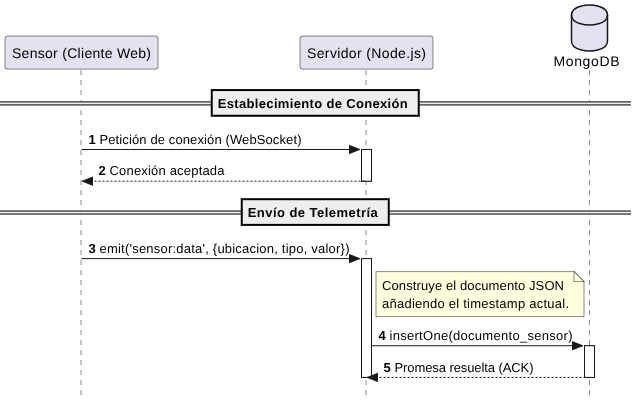
\includegraphics[width=0.85\textwidth]{./imagenes_necesarias/ejemplos_ejecucion/parte_2/DS_registrar_sensor.png}
				\caption{Diagrama de secuencia: Registro y envío de primera telemetría.}
				\label{fig:seq_registrar_sensor}
			\end{figure}
	
		\subsection{Escenario 2: Evaluación y Envío de un Aviso (Alerta Crítica)}
			En este escenario, se ilustra la intervención del Motor de Reglas (el Agente Lógico). Al recibir un dato que supera los umbrales de seguridad (por ejemplo, un nivel de gas excesivamente alto), el servidor ejecuta dos acciones concurrentes tras persistir el dato: emite un evento de \textit{broadcast} masivo para que todos los Dashboards conectados parpadeen con la alerta, y simultáneamente realiza una petición HTTP hacia la API de Telegram para notificar al dueño en su teléfono móvil.
		
			\begin{figure}[H]
				\centering
				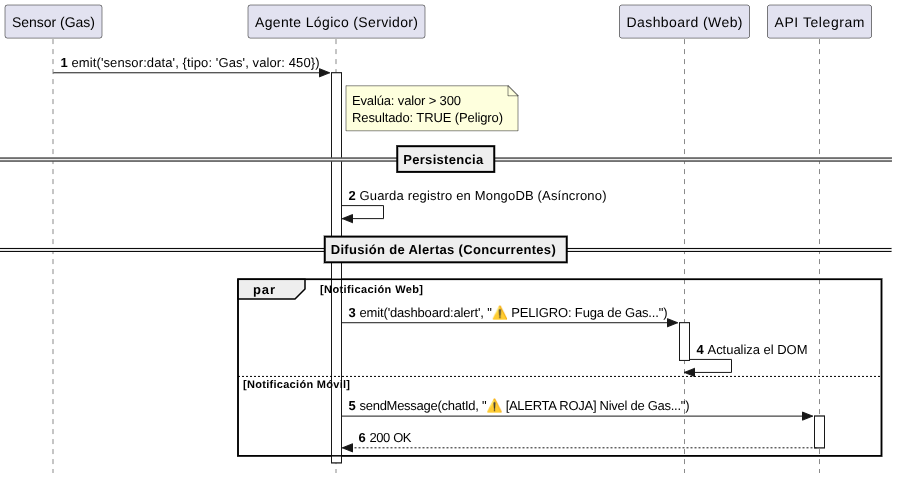
\includegraphics[width=0.85\textwidth]{./imagenes_necesarias/ejemplos_ejecucion/parte_2/DS_enviar_aviso.png}
				\caption{Diagrama de secuencia: Evaluación de reglas lógicas y difusión concurrente de alertas.}
				\label{fig:seq_enviar_aviso}
			\end{figure}
		
		\subsection{Escenario 3: Envío de Videovigilancia (Bypass Multimedia)}
			Este es un caso especial dentro de nuestra lógica de control. Cuando la cámara del portal detecta movimiento, el aviso en el Dashboard local es inmediato. Sin embargo, para la alerta externa, el servidor no envía el archivo de vídeo completo desde su propia memoria, sino que hace un \textit{bypass}: le envía a la API de Telegram la URL directa de un CDN de imágenes (Giphy). Es la propia infraestructura de Telegram la que se encarga de descargar el archivo pesado y entregárselo al usuario final, ahorrando así ancho de banda en nuestro servidor domótico.
			
			\begin{figure}[H]
				\centering
				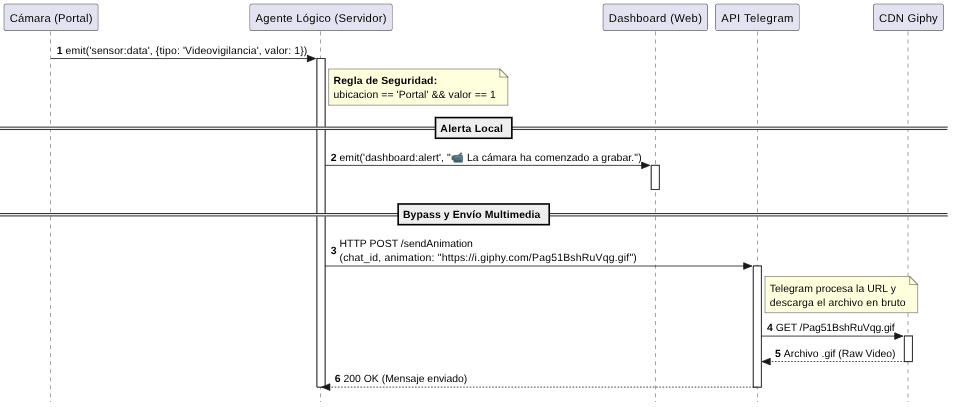
\includegraphics[width=0.9\textwidth]{./imagenes_necesarias/ejemplos_ejecucion/parte_2/DS_videovigilancia.png}
				\caption{Diagrama de secuencia: Integración de alertas multimedia y consumo de CDN externo.}
				\label{fig:seq_videovigilancia}
			\end{figure}

	\section{Guía de Uso y Ejemplos de Ejecución}
		Para poner en marcha el sistema domótico y comprobar su correcto funcionamiento, se ha preparado esta guía práctica paso a paso. El objetivo es detallar desde el encendido inicial de los servicios hasta la simulación de situaciones críticas para ver cómo reacciona nuestro ecosistema distribuido en tiempo real.
		
		\subsection{Puesta en Marcha del Sistema}
			En primer lugar, me gustaría comentar que, la práctica la he desarrollado en mi ordenador personal, que cuenta con las siguientes características:
			
			\begin{itemize}
				\item \textbf{Procesador (CPU):} 11th Gen Intel i5-1135G7.
				\item \textbf{Memoria RAM:} 16 GB DDR4.
				\item \textbf{Sistema Operativo:} Ubuntu 24.04.4 LTS x86\_64.
			\end{itemize}
			
			Para arrancar el proyecto, debemos seguir un orden lógico para asegurar que las conexiones entre los componentes (servidor, base de datos y clientes) se establezcan sin errores:
		
			\begin{enumerate}
				\item \textbf{Iniciar la Base de Datos:} Lo primero es comprobar que el servicio de MongoDB está corriendo en nuestra máquina local en el puerto por defecto (\texttt{27017}). Esto se hace abriendo una terminal y ejecutando:
				\begin{verbatim}
					$ sudo systemctl status mongod
				\end{verbatim}
				Si está corriendo ¡Perfecto! Ya puedes pasar al siguiente apartado. En caso contrario, arrancamos MongoDB con el siguiente comando: 
				\begin{verbatim}
					$ sudo systemctl start mongod
				\end{verbatim}

				\item \textbf{Encender el Servidor Central (Backend):} En una nueva ventana de la terminal, nos situamos en la carpeta del proyecto y lanzamos nuestro script de Node.js. Al hacerlo, la consola nos confirmará que se ha conectado con éxito a MongoDB y que el servidor web ya está escuchando peticiones:
				\begin{verbatim}
					$ node registro_sensores.js
				\end{verbatim}
		
				\item \textbf{Vincular DomoBot Angel:} Antes de abrir las webs, buscamos a nuestro bot en la aplicación de Telegram de nuestro móvil u ordenador y pulsamos el botón de \textbf{Iniciar} (lo que envía el comando \texttt{/start}). Veremos que la consola del servidor detecta el evento y registra nuestro \textit{Chat ID} para el envío de alertas. \textbf{Importante:} Tendremos que crearnos nosotros nuestro BOT y poner el token en la constante creada para ello en el Servidor (en \texttt{registro\_sensores.js})
			\end{enumerate}
	
		\subsection{Uso de las Interfaces de Usuario}
			Con el núcleo del sistema en marcha, abrimos nuestro navegador web e interactuamos con los dos clientes disponibles:
			
			\begin{itemize}
				\item \textbf{Simulador de Sensores:} (Figura~\ref{fig:panel_sensor}) Accedemos a la URL \texttt{http://localhost:8080/} (o \texttt{/sensor.html}). Desde aquí podemos dar de alta un sensor rellenando el formulario o seleccionar uno ya existente del desplegable. Si activamos el "Modo Piloto Automático", el cliente empezará a mandar datos inventados pero realistas cada 5 segundos de forma ininterrumpida.
				
				\begin{figure}[H]
					\centering
					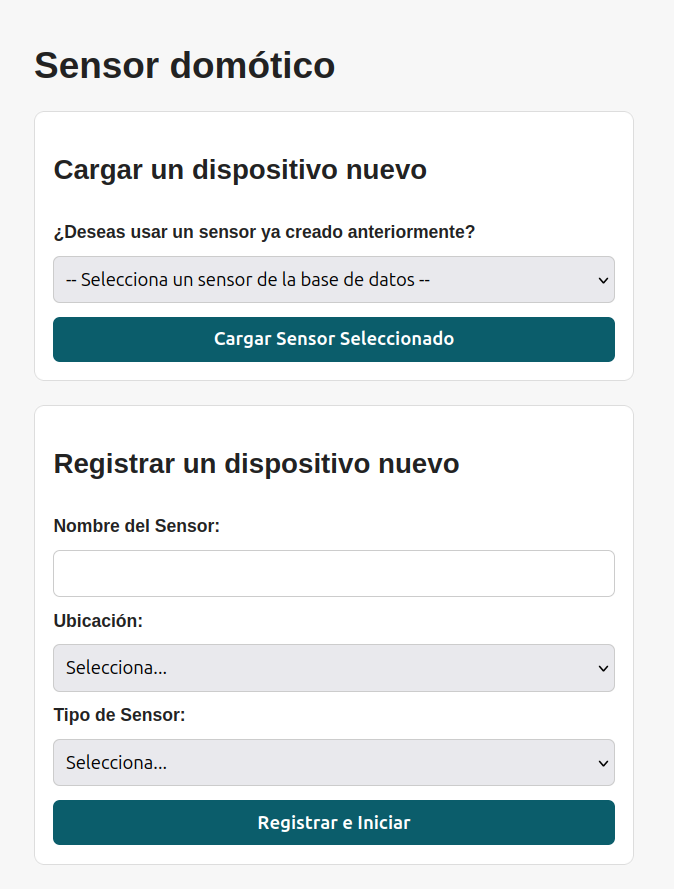
\includegraphics[width=0.7\linewidth]{./imagenes_necesarias/ejemplos_ejecucion/parte_2/Panel_sensor.png}
					\caption{Panel de registro de un sensor \texttt{http://localhost:8080/}}
					\label{fig:panel_sensor}
				\end{figure}
		
				\item \textbf{Panel de Control (Dashboard):} (Figura ~\ref{fig:dashboard}) En otra pestaña del navegador, entramos en \texttt{http://localhost:8080/dashboard.html}. Veremos cómo se dibuja la casa dinámicamente gracias al Gemelo Digital y cómo las tarjetas de cada habitación empiezan a actualizarse solas con las medidas que envía el simulador, sin necesidad de refrescar la página.
					
					\begin{figure}[H]
						\centering
						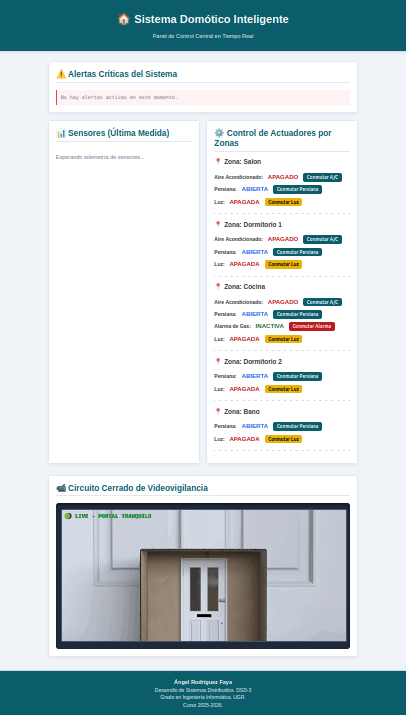
\includegraphics[width=1\linewidth]{./imagenes_necesarias/ejemplos_ejecucion/parte_2/Dashboard.png}
						\caption{Dashboard de un usuario/habitante de la casa domotizada \texttt{http://localhost:8080/dashboard.html}}
						\label{fig:dashboard}
					\end{figure}
				
				\item \textbf{Iniciar el bot de Telegram}: Le mandamos el comando \texttt{/start} (Figura ~\ref{fig:inicio_bot})
				
					\begin{figure}[H]
						\centering
						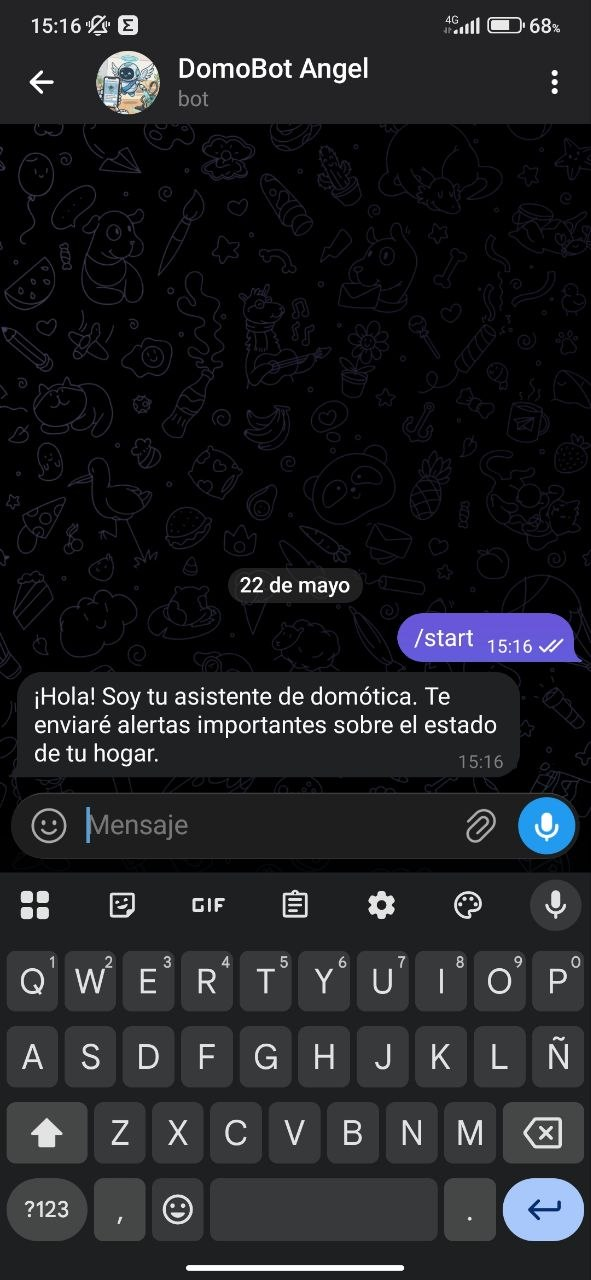
\includegraphics[width=0.4\linewidth]{./imagenes_necesarias/ejemplos_ejecucion/parte_2/inicio_bot.jpg}
						\caption{Inicio de conversación con DomoBot Angel}
						\label{fig:inicio_bot}
					\end{figure}
					
			\end{itemize}
	
		\subsection{Ejemplos de Ejecución y Casos de Prueba}
			Para demostrar el comportamiento inteligente del Agente Lógico y la perfecta sincronización de los clientes, vamos a ver cada uno de los pan exponen tres casos de prueba reales:
			
			\subsubsection{Caso de Prueba 1: Alerta Crítica por Fuga de Gas en la Cocina}
				En primer lugar registramos el \textbf{sensor de gas en la cocina} (Figuras ~\ref{fig:p1_1} y ~\ref{fig:p1_2}). 
				
				\begin{figure}[H]
					\centering
					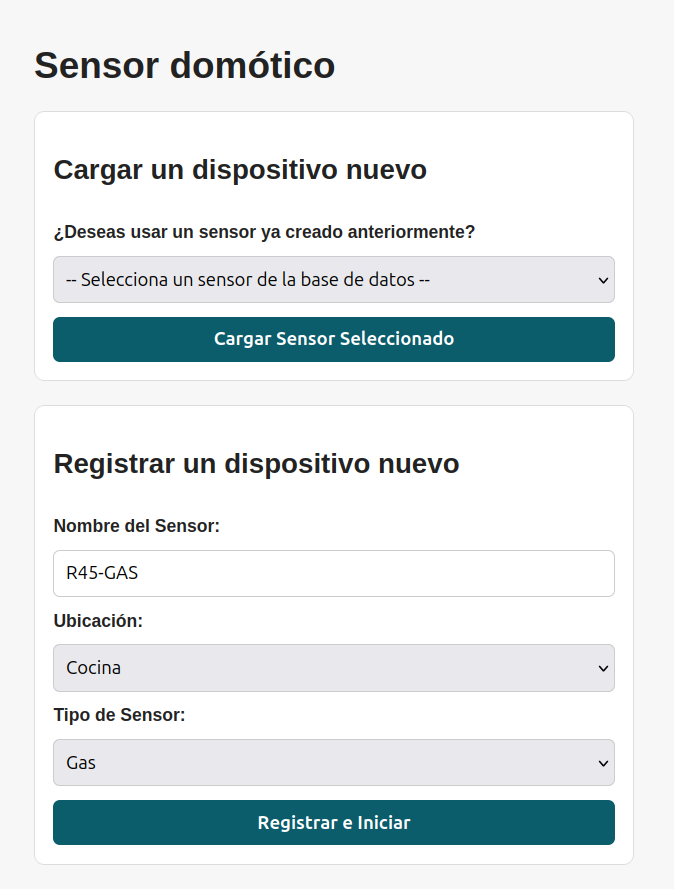
\includegraphics[width=0.7\linewidth]{./imagenes_necesarias/ejemplos_ejecucion/parte_2/prueba_1/1.png}
					\caption{Registramos un sensor de gas para la cocina.}
					\label{fig:p1_1}
				\end{figure}
				
				\begin{figure}[H]
					\centering
					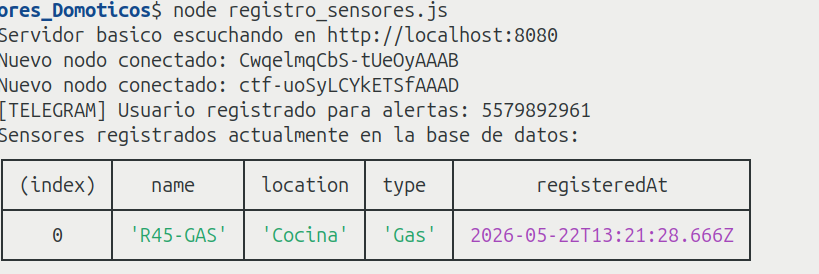
\includegraphics[width=0.7\linewidth]{./imagenes_necesarias/ejemplos_ejecucion/parte_2/prueba_1/2.png}
					\caption{Salida en la terminal al registrar un sensor de gas para la cocina.}
					\label{fig:p1_2}
				\end{figure}
				
				\begin{figure}[H]
					\centering
					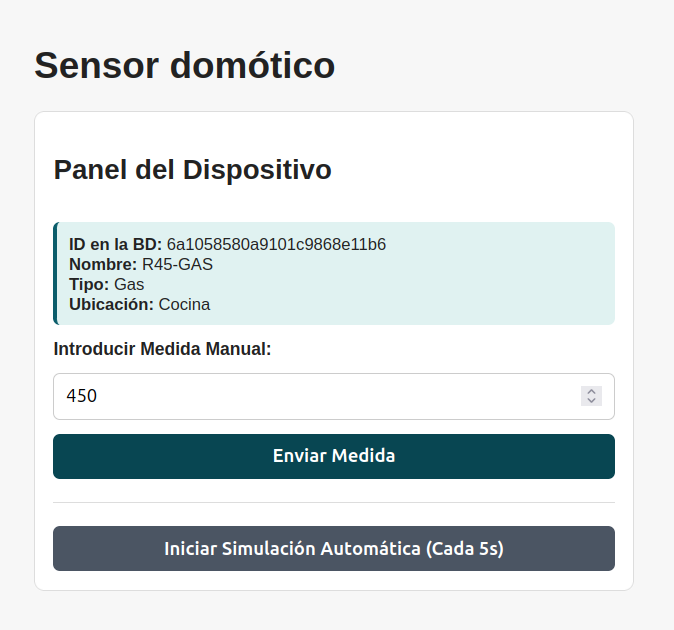
\includegraphics[width=0.7\linewidth]{./imagenes_necesarias/ejemplos_ejecucion/parte_2/prueba_1/3.png}
					\caption{Insertamos una medida de 450ppm para el sensor de gas para la cocina.}
					\label{fig:p1_3}
				\end{figure}
				
				\begin{figure}[H]
					\centering
					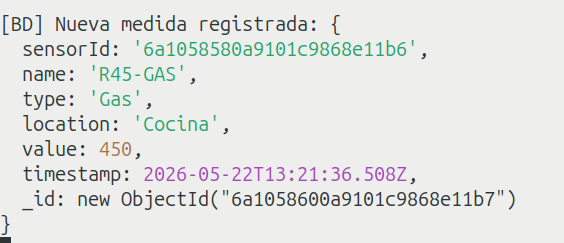
\includegraphics[width=0.7\linewidth]{./imagenes_necesarias/ejemplos_ejecucion/parte_2/prueba_1/4.png}
					\caption{Salida en la terminal al insertar una medida de 450ppm para el sensor de gas para la cocina.}
					\label{fig:p1_4}
				\end{figure}
				
				Si desde la interfaz del sensor inyectamos un valor de gas superior a las 300 ppm (por ejemplo, 450 ppm) (Figuras ~\ref{fig:p1_3} y  ~\ref{fig:p1_4} ) en la ubicación de la cocina, ocurre la siguiente reacción en cadena instantánea:
				\begin{itemize}
					\item El servidor persiste la lectura en la colección \texttt{historial} de MongoDB. Ya lo hemos visto en la Figura ~\ref{fig:p1_4} 
					\item El \textit{Dashboard} intercepta el aviso (Figura ~\ref{fig:p1_5}), añade una alerta roja en el historial de pantallas y conmuta de forma automática el estado de la Alarma de Gas de la cocina a \texttt{ACTIVA}.
						\begin{figure}[H]
							\centering
							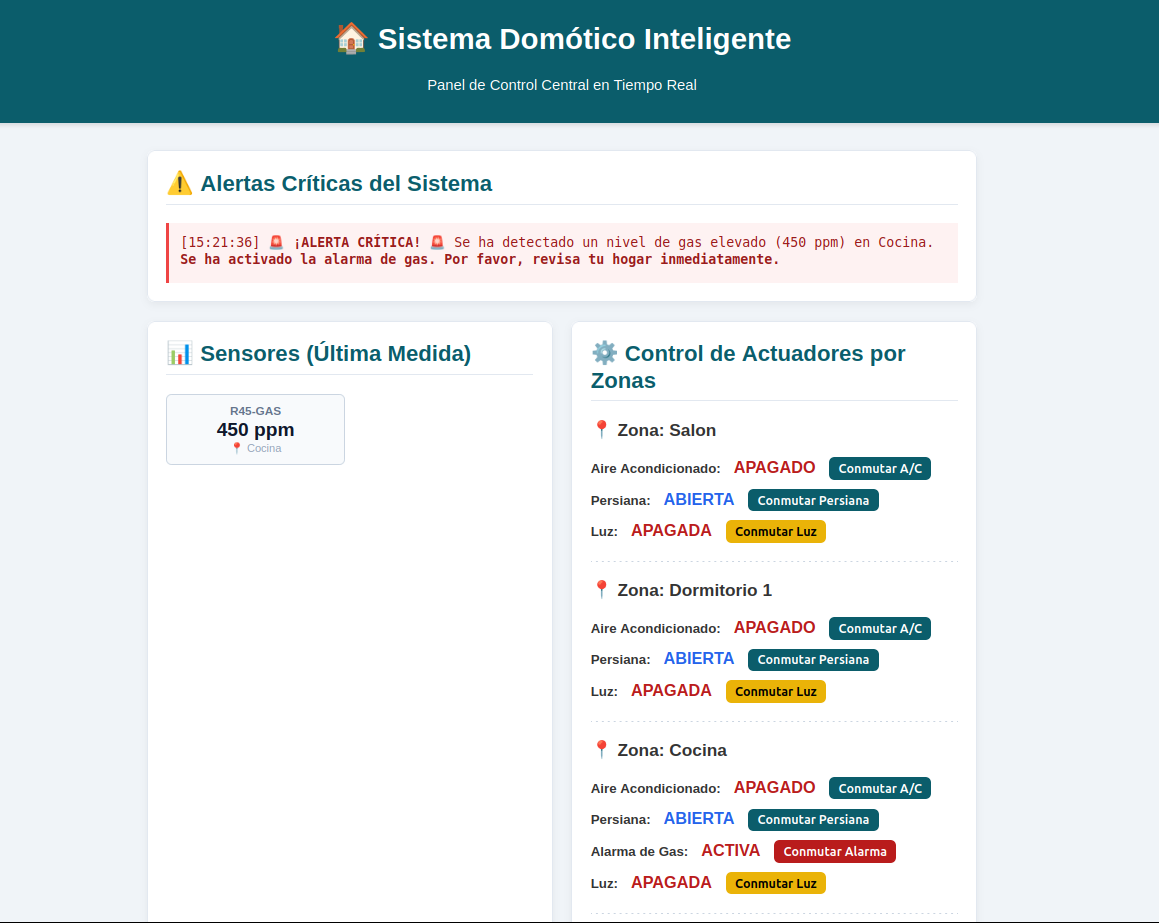
\includegraphics[width=1\linewidth]{./imagenes_necesarias/ejemplos_ejecucion/parte_2/prueba_1/5.png}
							\caption{Dashboard muestra el aviso de fuga de gas detectado por el sensor de la cocina}
							\label{fig:p1_5}
						\end{figure}
					\item El usuario recibe una notificación en su teléfono móvil mediante Telegram advirtiéndole del peligro de forma inmediata (Figura ~\ref{fig:p1_6}).
						\begin{figure}[H]
							\centering
							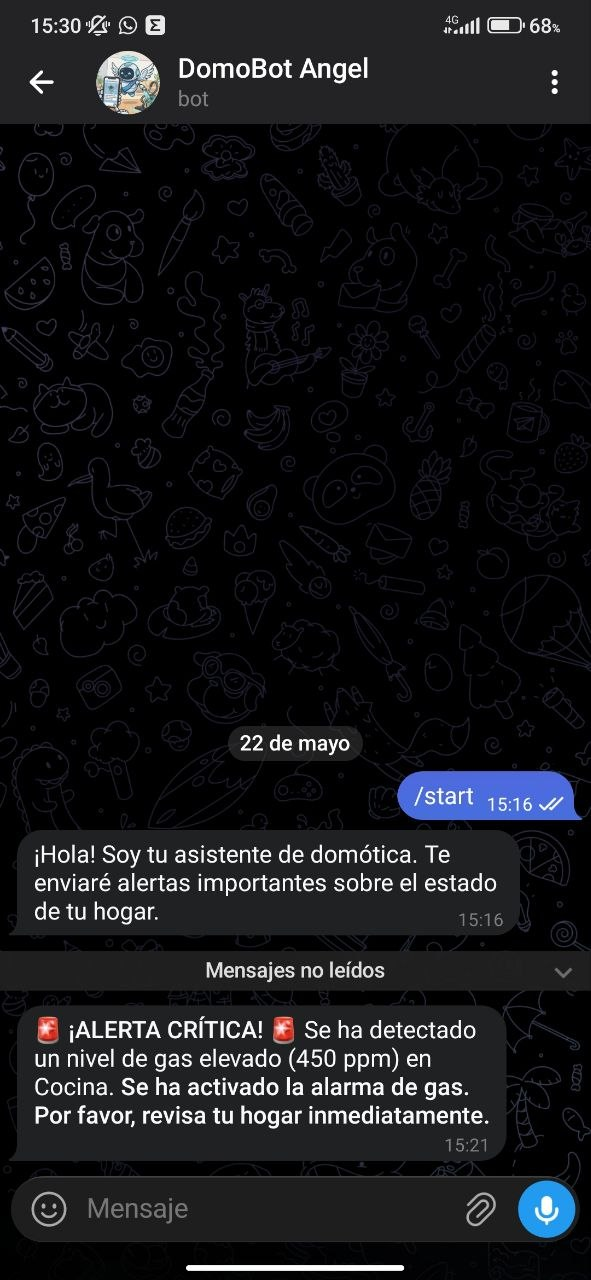
\includegraphics[width=0.4\linewidth]{./imagenes_necesarias/ejemplos_ejecucion/parte_2/prueba_1/6.jpg}
							\caption{DomoBot Angel nos avisa de la fuga de gas detectado por el sensor de la cocina}
							\label{fig:p1_6}
						\end{figure}
				\end{itemize}
				
			\newpage
		\subsubsection{Caso de Prueba 2: Regla Compleja Cruzada (Luminosidad y Movimiento)}
				Para comprobar que el Agente Lógico tiene memoria asociativa y toma decisiones eficientes, realizamos la siguiente prueba:
				\begin{enumerate}
					\item Enviamos desde un sensor una lectura de \texttt{Luminosidad} alta (por ejemplo, 600 lux) en el \texttt{Salón}. Acto seguido, simulamos presencia (\texttt{1}) con un sensor de \texttt{Movimiento} en esa misma zona (Figura ~\ref{fig:p2_1}). El servidor registra el movimiento, pero como sabe que hay luz de día, decide no hacer nada. (Figura ~\ref{fig:p2_2})
					
					\begin{figure}[H]
						\centering
						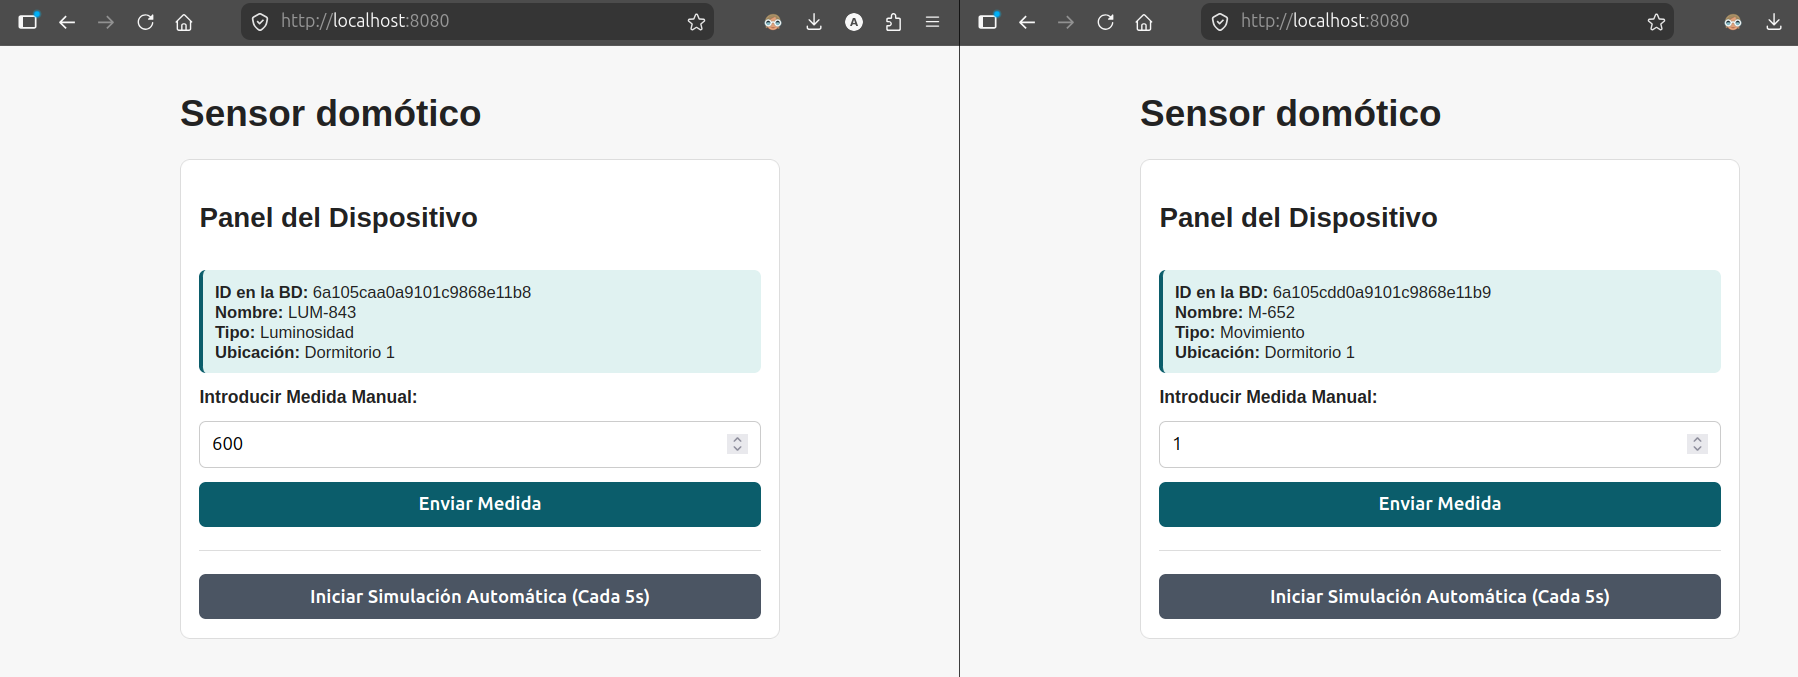
\includegraphics[width=1\linewidth]{./imagenes_necesarias/ejemplos_ejecucion/parte_2/prueba_2/1.png}
						\caption{Sensor de Luminosidad y Movimiento en Dormitorio 1 envían su telemetría}
						\label{fig:p2_1}
					\end{figure}
					
					\begin{figure}[H]
						\centering
						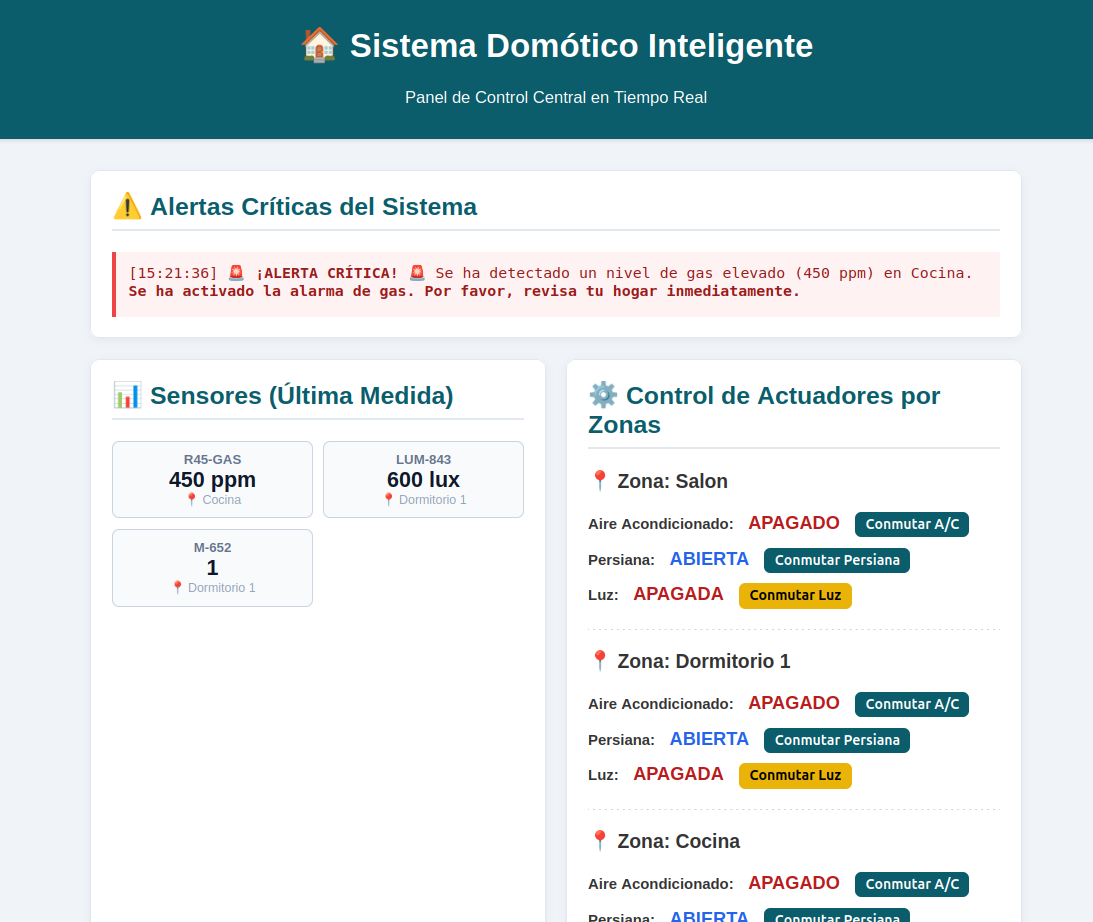
\includegraphics[width=1\linewidth]{./imagenes_necesarias/ejemplos_ejecucion/parte_2/prueba_2/2.png}
						\caption{Dashboard con nuevas telemetrías}
						\label{fig:p2_2}
					\end{figure}
				
				\item Ahora (Figura ~\ref{fig:p2_3}), cambiamos la \texttt{Luminosidad} a un valor bajo (por ejemplo, 80 lux) simulando que ha anochecido. Volvemos a mandar un evento de \texttt{Movimiento}. Al cruzar ambos datos en memoria, el Agente determina que está oscuro y hay presencia, por lo que cambia el estado de la Luz del Salón a \texttt{ENCENDIDA} en el Gemelo Digital, el botón del Dashboard (Figura ~\ref{fig:p2_4}) cambia de color solo y nos llega el aviso. DomoBot Angel también nos avisa (Figura ~\ref{fig:p2_5})
				
					\begin{figure}[H]
						\centering
						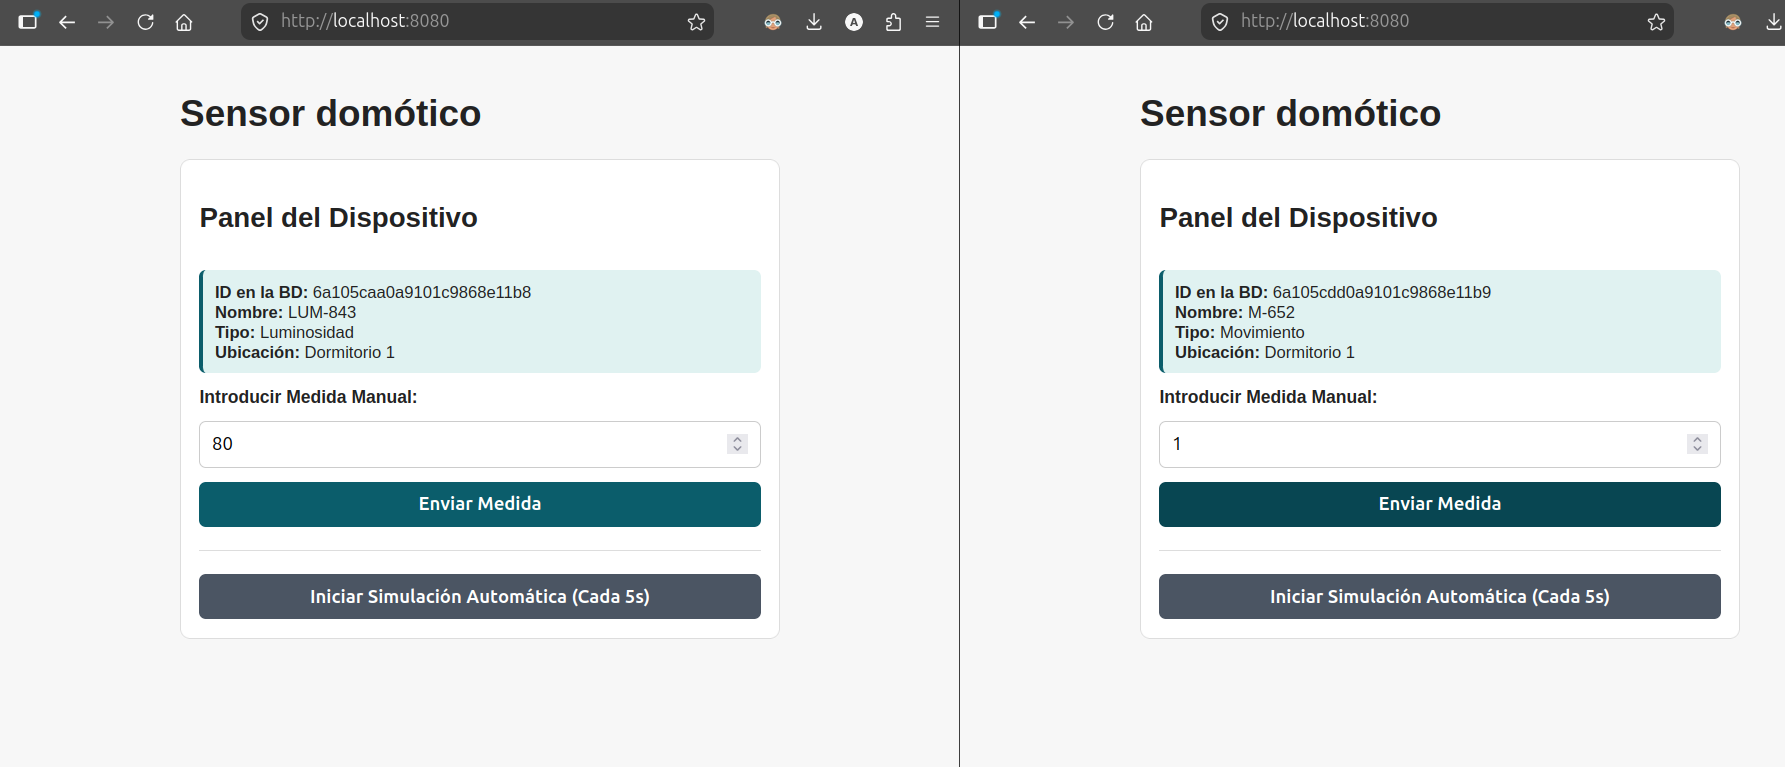
\includegraphics[width=1\linewidth]{./imagenes_necesarias/ejemplos_ejecucion/parte_2/prueba_2/3.png}
						\caption{Sensor de Luminosidad y Movimiento en Dormitorio 1 envían su telemetría de nuevo}
						\label{fig:p2_3}
					\end{figure}
					
					\begin{figure}[H]
						\centering
						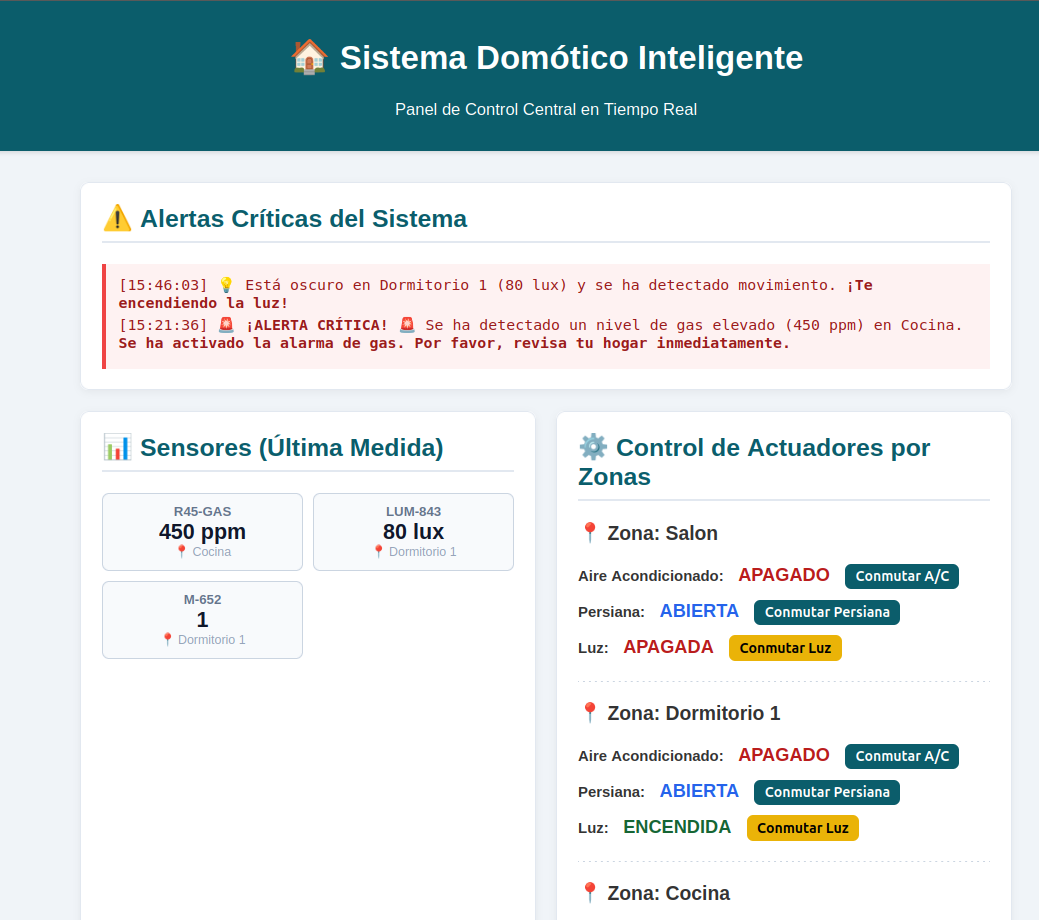
\includegraphics[width=1\linewidth]{./imagenes_necesarias/ejemplos_ejecucion/parte_2/prueba_2/4.png}
						\caption{Dashboard con nuevas telemetrías, nuevo aviso y cambio en el actuador de la Luz del Dormitorio 1.}
						\label{fig:p2_4}
					\end{figure}
					
					\begin{figure}[H]
						\centering
						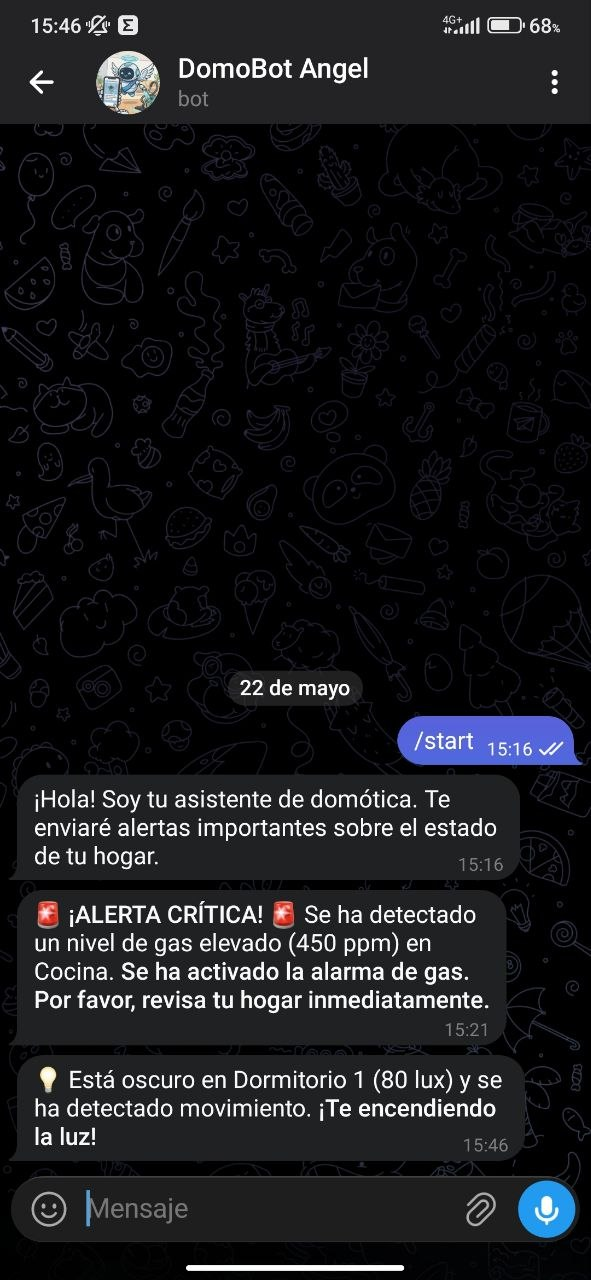
\includegraphics[width=0.4\linewidth]{./imagenes_necesarias/ejemplos_ejecucion/parte_2/prueba_2/5.jpg}
						\caption{DomoBot Angel nos avisa de que ha enendido la luz debido al evento complejo}
						\label{fig:p2_5}
					\end{figure}
					
			\end{enumerate}
		
		\newpage
		
		\subsubsection{Caso de Prueba 3: Seguridad en el Portal (Videovigilancia Activa)}
			Cuando el sensor de \texttt{Videovigilancia} del \texttt{Portal} detecta actividad (Figura  ~\ref{fig:p3_1}) (un valor igual a \texttt{1}), el sistema se pone en modo alerta de seguridad:
				\begin{figure}[H]
					\centering
					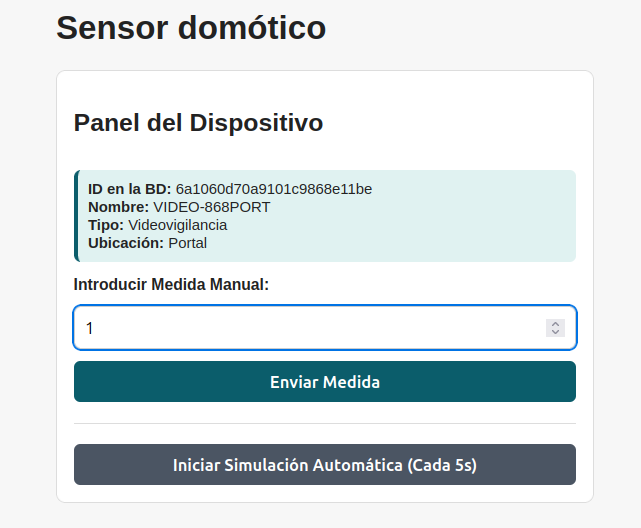
\includegraphics[width=1\linewidth]{./imagenes_necesarias/ejemplos_ejecucion/parte_2/prueba_3/1.png}
					\caption{El sensor de Videovigilancia ubicado en el Portal detecta movimiento}
					\label{fig:p3_1}
				\end{figure}
				
			\begin{itemize}
				\item El \textit{Dashboard} reacciona (de la Figura  ~\ref{fig:p3_2}) cambiando el estilo del circuito cerrado de videovigilancia (CCV) (Figura ~\ref{fig:p3_3}), sustituyendo la imagen estática por una animación interactiva con un marco rojo que simula que la cámara está grabando al intruso.
					\begin{figure}[H]
						\centering
						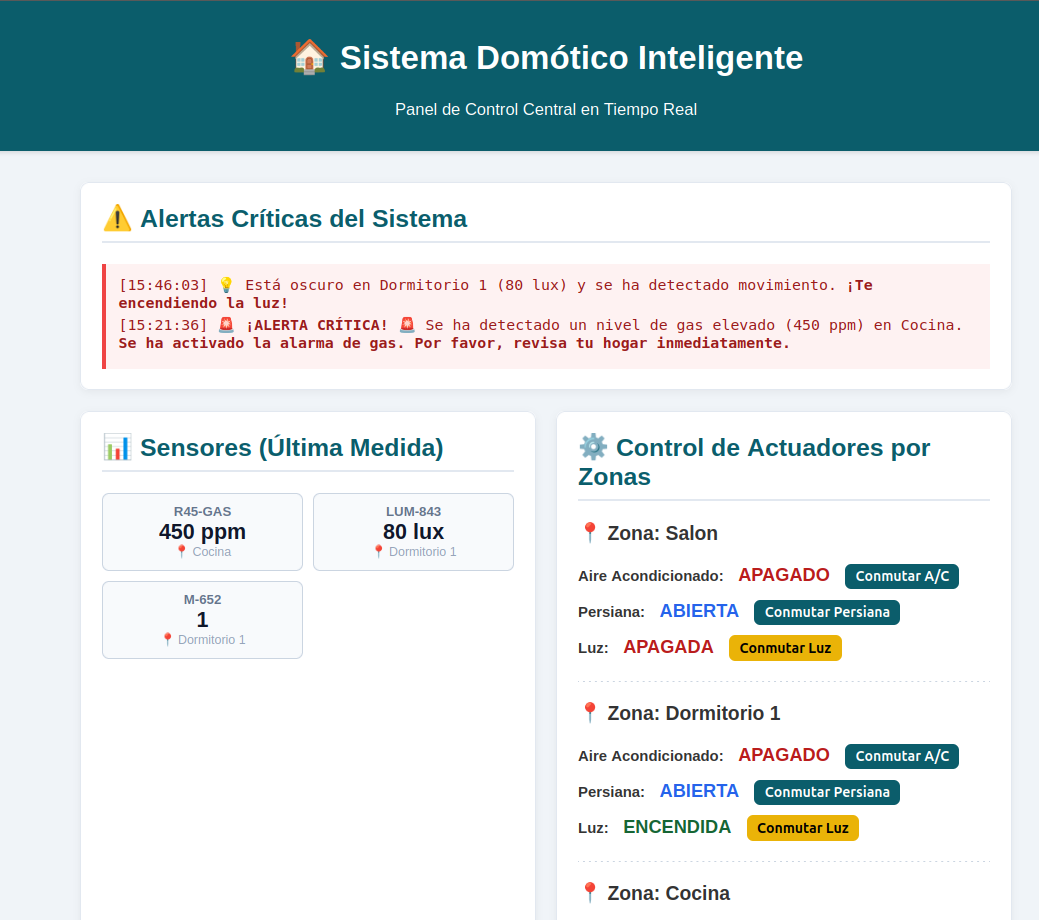
\includegraphics[width=1\linewidth]{./imagenes_necesarias/ejemplos_ejecucion/parte_2/prueba_2/4.png}
						\caption{CCV normal, sin detectar movimiento.}
						\label{fig:p3_2}
					\end{figure}
					
					\begin{figure}[H]
						\centering
						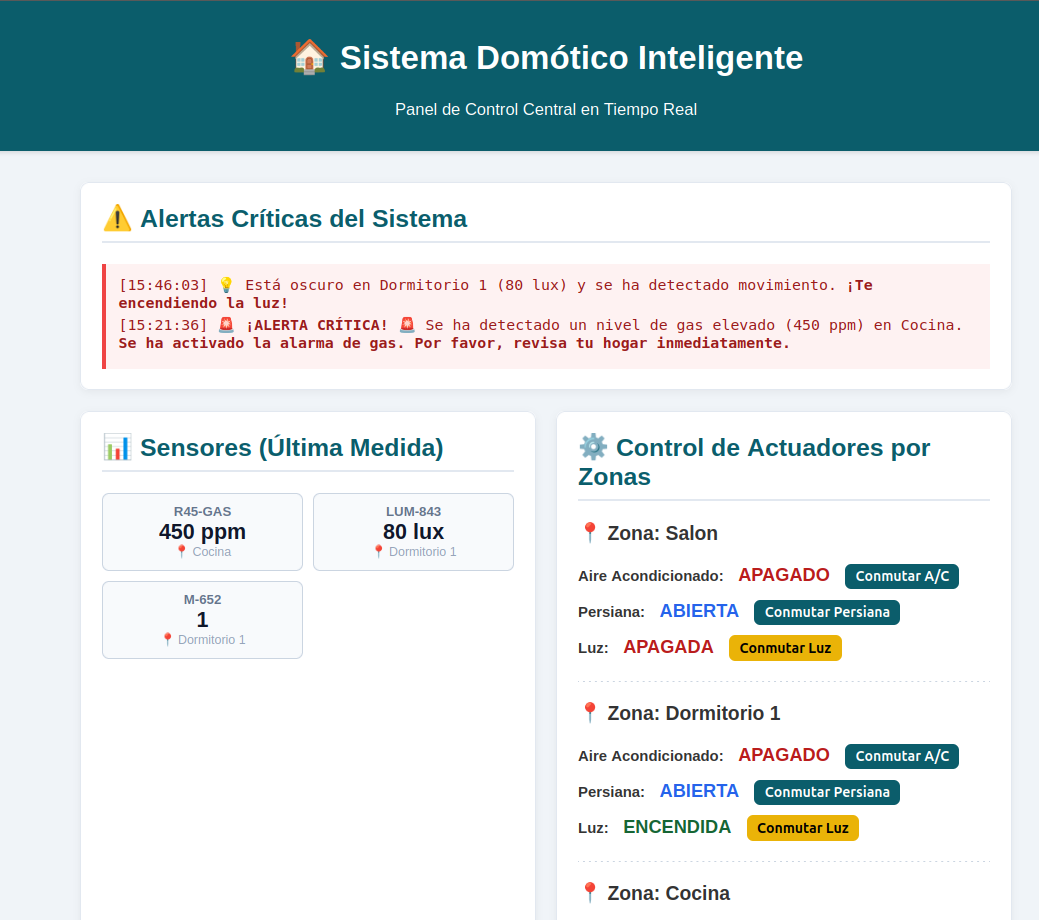
\includegraphics[width=1\linewidth]{./imagenes_necesarias/ejemplos_ejecucion/parte_2/prueba_2/4.png}
						\caption{CCV al detectar movimiento.}
						\label{fig:p3_3}
					\end{figure}
					
				\item El servidor realiza el \textit{bypass} multimedia y le envía al usuario por Telegram un mensaje HTML junto con un GIF animado en tiempo real, permitiendo al dueño ver una simulación visual de lo que ocurre en su puerta desde cualquier parte del mundo.  (Figura ~\ref{fig:p3_4})
					\begin{figure}[H]
						\centering
						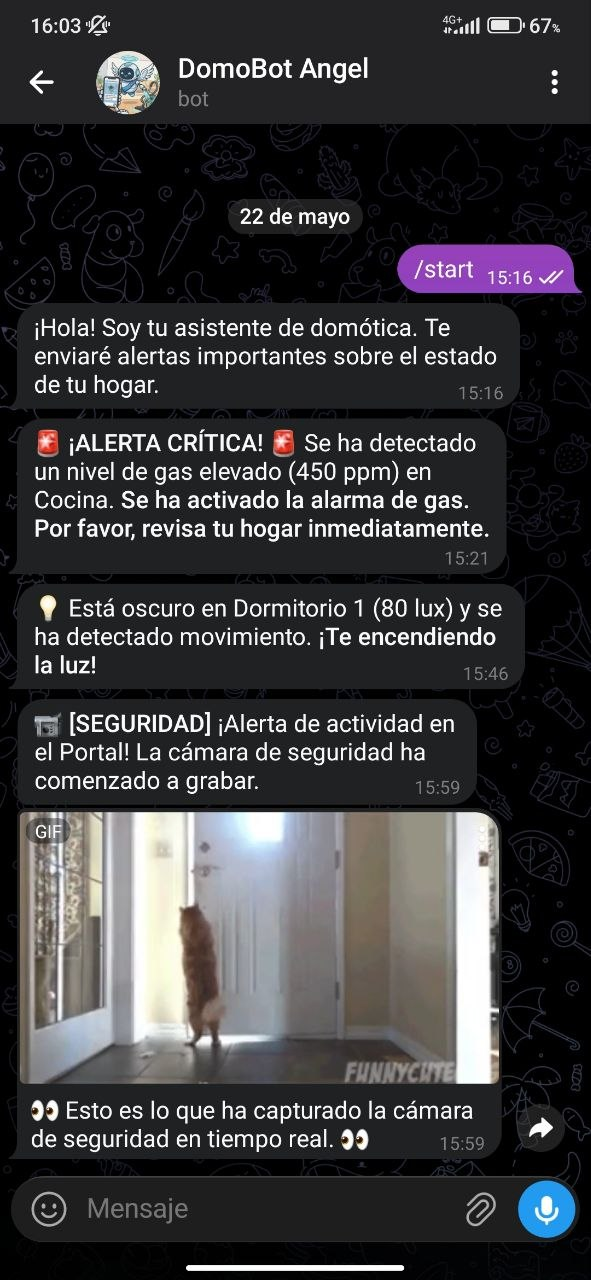
\includegraphics[width=0.4\linewidth]{./imagenes_necesarias/ejemplos_ejecucion/parte_2/prueba_3/4.jpg}
						\caption{DomoBot Angel nos avisa de que hay alguien en el portal y nos envia un pequeño clip de lo que graban las cámaras}
						\label{fig:p3_4}
					\end{figure}
			\end{itemize}
			
				
\end{document}